\ifx\allfiles\undefined
\documentclass[12pt, a4paper,oneside, UTF8]{ctexbook}
\usepackage[dvipsnames]{xcolor}
\usepackage{amsmath}   % 数学公式
\usepackage{amsthm}    % 定理环境
\usepackage{amssymb}   % 更多公式符号
\usepackage{graphicx}  % 插图
%\usepackage{mathrsfs}  % 数学字体
%\usepackage{newtxtext,newtxmath}
%\usepackage{arev}
\usepackage{kmath,kerkis}
\usepackage{enumitem}  % 列表
\usepackage{geometry}  % 页面调整
%\usepackage{unicode-math}
\usepackage[colorlinks,linkcolor=black]{hyperref}


\usepackage{ulem}	   % 用于更多的下划线格式,
					   % \uline{}下划线,\uuline{}双下划线,\uwave{}下划波浪线,\sout{}中间删除线,\xout{}斜删除线
					   % \dashuline{}下划虚线,\dotuline{}文字底部加点


\graphicspath{ {flg/},{../flg/}, {config/}, {../config/} }  % 配置图形文件检索目录
\linespread{1.5} % 行高

% 页码设置
\geometry{top=25.4mm,bottom=25.4mm,left=20mm,right=20mm,headheight=2.17cm,headsep=4mm,footskip=12mm}

% 设置列表环境的上下间距
\setenumerate[1]{itemsep=5pt,partopsep=0pt,parsep=\parskip,topsep=5pt}
\setitemize[1]{itemsep=5pt,partopsep=0pt,parsep=\parskip,topsep=5pt}
\setdescription{itemsep=5pt,partopsep=0pt,parsep=\parskip,topsep=5pt}

% 定理环境
% ########## 定理环境 start ####################################
\theoremstyle{definition}
\newtheorem{defn}{\indent 定义}[section]

\newtheorem{lemma}{\indent 引理}[section]    % 引理 定理 推论 准则 共用一个编号计数
\newtheorem{thm}[lemma]{\indent 定理}
\newtheorem{corollary}[lemma]{\indent 推论}
\newtheorem{criterion}[lemma]{\indent 准则}

\newtheorem{proposition}{\indent 命题}[section]
\newtheorem{example}{\indent \color{SeaGreen}{例}}[section] % 绿色文字的 例 ,不需要就去除\color{SeaGreen}{}
\newtheorem*{rmk}{\indent \color{red}{注}}

% 两种方式定义中文的 证明 和 解 的环境:
% 缺点:\qedhere 命令将会失效【技术有限,暂时无法解决】
\renewenvironment{proof}{\par\textbf{证明.}\;}{\qed\par}
\newenvironment{solution}{\par{\textbf{解.}}\;}{\qed\par}

% 缺点:\bf 是过时命令,可以用 textb f等替代,但编译会有关于字体的警告,不过不影响使用【技术有限,暂时无法解决】
%\renewcommand{\proofname}{\indent\bf 证明}
%\newenvironment{solution}{\begin{proof}[\indent\bf 解]}{\end{proof}}
% ######### 定理环境 end  #####################################

% ↓↓↓↓↓↓↓↓↓↓↓↓↓↓↓↓↓ 以下是自定义的命令  ↓↓↓↓↓↓↓↓↓↓↓↓↓↓↓↓

% 用于调整表格的高度  使用 \hline\xrowht{25pt}
\newcommand{\xrowht}[2][0]{\addstackgap[.5\dimexpr#2\relax]{\vphantom{#1}}}

% 表格环境内长内容换行
\newcommand{\tabincell}[2]{\begin{tabular}{@{}#1@{}}#2\end{tabular}}

% 使用\linespread{1.5} 之后 cases 环境的行高也会改变,重新定义一个 ca 环境可以自动控制 cases 环境行高
\newenvironment{ca}[1][1]{\linespread{#1} \selectfont \begin{cases}}{\end{cases}}
% 和上面一样
\newenvironment{vx}[1][1]{\linespread{#1} \selectfont \begin{vmatrix}}{\end{vmatrix}}

\def\d{\textup{d}} % 直立体 d 用于微分符号 dx
\def\R{\mathbb{R}} % 实数域
\def\N{\mathbb{N}} % 自然数域
\def\C{\mathbb{C}} % 复数域
\def\Z{\mathbb{Z}} % 整数环
\def\Q{\mathbb{Q}} % 有理数域
\newcommand{\bs}[1]{\boldsymbol{#1}}    % 加粗,常用于向量
\newcommand{\ora}[1]{\overrightarrow{#1}} % 向量

% 数学 平行 符号
\newcommand{\pll}{\kern 0.56em/\kern -0.8em /\kern 0.56em}

% 用于空行\myspace{1} 表示空一行 填 2 表示空两行  
\newcommand{\myspace}[1]{\par\vspace{#1\baselineskip}}

%s.t. 用\st就能打出s.t.
\DeclareMathOperator{\st}{s.t.}

%罗马数字 \rmnum{}是小写罗马数字, \Rmnum{}是大写罗马数字
\makeatletter
\newcommand{\rmnum}[1]{\romannumeral #1}
\newcommand{\Rmnum}[1]{\expandafter@slowromancap\romannumeral #1@}
\makeatother
\begin{document}
	% \title{{\Huge{\textbf{$Basic \,\, Topology$\footnote{课堂教材:\textbf{《基础拓扑学讲义》——尤承业}}}}}}
\author{$-TW-$}
\date{\today}
\maketitle                   % 在单独的标题页上生成一个标题

\thispagestyle{empty}        % 前言页面不使用页码
\begin{center}
	\Huge\textbf{序}
\end{center}


\vspace*{3em}
\begin{center}
	\large{\textbf{天道几何,万品流形先自守;}}\\
	
	\large{\textbf{变分无限,孤心测度有同伦。}}
\end{center}

\vspace*{3em}
\begin{flushright}
	\begin{tabular}{c}
		\today \\ \small{\textbf{长夜伴浪破晓梦,梦晓破浪伴夜长}}
	\end{tabular}
\end{flushright}


\newpage                      % 新的一页
\pagestyle{plain}             % 设置页眉和页脚的排版方式(plain:页眉是空的,页脚只包含一个居中的页码)
\setcounter{page}{1}          % 重新定义页码从第一页开始
\pagenumbering{Roman}         % 使用大写的罗马数字作为页码
\tableofcontents              % 生成目录

\newpage                      % 以下是正文
\pagestyle{plain}
\setcounter{page}{1}          % 使用阿拉伯数字作为页码
\pagenumbering{arabic}
\setcounter{chapter}{0}    % 设置 -1 可作为第零章绪论从第零章开始 
	\else
	\fi
	%  ############################ 正文部分
\chapter{拓扑空间和连续性}

\section{拓扑空间}
\subsection{度量拓扑}
\paragraph{定义}
	下面给出度量空间$X$ 的定义:
	\begin{defn}\label{def 1.1.1}
		集合$X$ 上的度量$d$ 是一个映射$d : X \times X \longrightarrow \R , \st$
		\begin{enumerate}
			\item[\rmnum{1}] 正定性:
			\begin{align}
				d(x , y) \geq 0 , \forall x , y \in X \hspace*{3em} "=" \Leftrightarrow x = y
			\end{align}
			
			\item[\rmnum{2}] 对称性:
			\begin{align}
				d(x , y) = d(y , x) , \forall x , y \in X
			\end{align}
		
			\item[\rmnum{3}] 三角不等式:
			\begin{align}
				d(x , y) \leq d(x , z) + d(z , y) , \forall x , y , z \in X
			\end{align}
		\end{enumerate}
		当集合$X$ 上规定了一个度量$d$ 后,称为\underline{\textbf{度量空间}},记作$(X , d)$
	\end{defn}
	
\paragraph{度量拓扑}
	设$(X , d)$ 为一个度量空间,下面规定$X$ 的一个拓扑。\\
	首先给出球形邻域(开球)的概念,此处的定义与欧氏空间中的一致
	\begin{defn}\label{def 1.1.2}
		设$x_0 \in X$,$\epsilon > 0$,称$X$ 的子集
		\begin{align}
			B(x_0 , \epsilon) \coloneqq \{ x \in X \mid d(x_0 , x) < \epsilon \}
		\end{align}
		为以$x_0$ 为心,$\epsilon$ 为半径的球形邻域(开球)
	\end{defn}

	接下来准备定义空间$X$ 上的度量拓扑
	\begin{lemma}\label{lemma 1.1.1}
		$(X , d)$ 的任意两个开球的交集是若干个开球的并
	\end{lemma}
	
	\begin{proof}
		$Suppose \,\, U = B(x_1 , \epsilon_1) \cap B(x_2 , \epsilon_2)$\\
		$\forall x \in U , \,\, let \,\, \epsilon_{x} = min\{ \epsilon_1 - d(x , x_1) , \,\, \epsilon_2 - d(x , x_2) \}$\\
		$Then \,\, for \,\, each \,\, y \in B(x , \,\, \epsilon_x) ,$
		\begin{align}
			d(y , x_1) &\leq d(y , x) + d(x , x_1) \leq \epsilon_1\\
			d(y , x_2) &\leq d(y , x) + d(x , x_2) \leq \epsilon_2
		\end{align}
		$Therefore , \,\, y \in U , \,\, \forall y \in B(x , \epsilon_x) , \,\, So \,\, B(x , \epsilon_x) \subseteq U$\\
		$Thus , $
		\begin{align}
			U = \bigcup_{x \in U}{B(x , \epsilon_x)}
		\end{align}
	\end{proof}

	\begin{proposition}\label{prop 1.1.1}
		设$X$ 的子集族
		\begin{align}
			\tau_d \coloneqq \{ U \mid U \text{为若干个开球的并} \}
		\end{align}
		则$\tau_d$ 为$X$ 上的一个拓扑,称为$X$ 上由度量$d$ 决定的\underline{\textbf{度量拓扑}}
	\end{proposition}

	\begin{proof}
		$\varnothing \in \tau_d , \,\, X = \bigcup_{x \in X}{B(x , \epsilon_x)}$\\
		显然$\tau_d$ 中的任意元素之并仍在$\tau_d$ 中\\
		$\forall U_1 , \,\, U_2 \in \tau_d , \,\, let \,\, U_1 = \bigcup_{\alpha \in I}{B(x_{\alpha} , \epsilon_{\alpha})} , \,\, U_2 = \bigcup_{\beta \in J}{B(x_{\beta} , \epsilon_{\beta})} , \,\, Then$
		\begin{align}
			U_1 \cap U_2 
			&= (\bigcup_{\alpha \in I}{B(x_{\alpha} , \epsilon_{\alpha})}) \cap 
			(\bigcup_{\beta \in J}{B(x_{\beta} , \epsilon_{\beta})})\\
			&= \bigcup_{\alpha \in I , \,\, \beta \in J}{B(x_{\alpha} , \epsilon_{\alpha}) \cap B(x_{\beta} , \epsilon_{\beta})}
		\end{align}
		$According \,\, to \,\, Lemma\ref{lemma 1.1.1} , \,\, U_1 \cap U_2 \in \tau_d$
	\end{proof}

\newpage

\subsection{序列的收敛性}
\paragraph{定义}
	首先回顾一下拓扑空间中的邻域以及数学分析中序列收敛的概念:
	\begin{defn}\label{def 1.1.3}
		设$A$ 是拓扑空间$X$ 的一个子集,点$x \in A$.如果存在开集$U$,满足$x \in U \subseteq A$,则称$x$ 是$A$ 的一个内点,$A$ 是$x$ 的一个\underline{\textbf{邻域}}.
	\end{defn}

	\begin{defn}\label{def 1.1.4}
		设$\{ x_n \}$ 为拓扑空间$X$ 中的点序列.如果点$x_0$ 的\uwave{\textbf{\textcolor{red}{任意}}邻域$U$}都包含$\{ x_n \}$的几乎所有项(即只有有限个$x_n$ 不在$U$ 中;或$\exists N \in \N , \,\, \st x_n \in U , \,\, \forall n > N$),\\
		称$\{ x_n \}$ \underline{\textbf{收敛}}到$x_0$,记作$x_n \to x_0$
	\end{defn}

\paragraph{举例}
	拓扑空间中推广的序列收敛的概念中失去了一些重要的性质.
	\begin{enumerate}
		\item 拓扑空间中的序列可能收敛到多个点.
		\begin{example}\label{ex 1.1.1}
			考虑$\R$ 上的余有限拓扑$(\R , \tau_f)$,只要序列$\{ x_n \}$ 的项两两不同,则任一点$x \in \R$ 的邻域(必是有限集的余集)包含$\{ x_n \}$ 的几乎所有项,从而$x_n \to x$
		\end{example}
	
		\begin{rmk}
			\begin{enumerate}
				\item[\rmnum{1}] $\R$ 上的余有限拓扑$(\R , \tau_f)$ 中,开集为有限集的余集,即可视作在数轴中挖去有限个点所剩下的集合
				
				\item[\rmnum{2}] 事实上条件“序列$\{ x_n \}$ 的项两两不同”可减弱为“序列$\{ x_n \}$ 中每一项都只出现有限次”
			\end{enumerate}
		\end{rmk}
	
		\item 可能出现$A$ 中任一序列均不收敛到聚点$x$ 的情况.
		\begin{example}\label{ex 1.1.2}
			考虑$\R$ 上的余可数拓扑$(\R , \tau_c)$,设$A = (0 , 1) , \,\, x_0 = 2$,则$x_0$ 的任一邻域$U$ 均包含$A$ 中元素,即$U \cap A \neq \varnothing$,所以$x_0$ 为$A$ 的聚点.但对于任一$A$ 中序列$\{ x_n \}$,其可看作可数集$M = \{ x_n \}$,于是集合$S = \R \backslash M$ 为开集,且为包含$x_0$ 的邻域,且$S$ 中不包含序列$\{ x_n \}$ 中任一项,从而$A$ 中序列$\{ x_n \}$ 并不收敛到聚点$x_0$
		\end{example}
	\end{enumerate}

\newpage
\subsection{拓扑基$Topology \,\, Basis$}
\paragraph{引入}
	回顾欧氏空间$\R^n$ 中的开集与开球之间的关系.
	\begin{align}
		U \underset{open}{\subseteq} \R^n &\Longleftrightarrow \forall p \in U , \,\, \exists \delta_p > 0 , \,\, \st B(p , \delta_p) \subseteq U\\
		U &= \bigcup_{p \in U}{B(p , \delta_p)}
	\end{align}
	其中每个开集都可由若干个开球$B(p , \delta_p)$ 组成,开球$B(p , \delta_p)$ 起到了\textbf{“砖块”}的作用.

\vspace*{2em}
\paragraph{定义}
	类比欧式空间中开球的性质,下面给出一般的拓扑空间中拓扑基的定义.
	\begin{defn}\label{def 1.1.5}
		设$X$ 为一个拓扑空间,$\mathcal{B}$ 为一个由$X$ 中若干个开集构成的集族.若$\forall \,\, X$ 中的开集$U$,$U$ 可表为$\mathcal{B}$ 中若干元素之并,即
		\begin{align}
			\forall U \underset{open}{\subseteq} X , \,\, U = \bigcup_{\alpha \in I}{U_\alpha} , \,\, U_\alpha \in \mathcal{B}
		\end{align}
		则称$\mathcal{B}$ 构成了$X$ 的一个\underline{\textbf{拓扑基($Topology \,\, Basis$)}}
	\end{defn}
	\begin{example}\label{ex 1.1.3}
		考虑$\R^1$ 欧式拓扑,则$\mathcal{B} = \{ (a , b) \mid a < b \}$ 为$\R$ 的一组拓扑基.\\
		令$\mathcal{B}^{'} = \{ (a , b) \mid a < b , \,\, a , b \in \Q \}$,则$\mathcal{B}^{'}$ 也为$\R$ 的一组拓扑基.
	\end{example}

	下面给出拓扑基的一个刻画.
	\begin{proposition}\label{prop 1.1.2}
		设$X$ 是一个集合,$\mathcal{B}$ 为$X$ 的若干子集构成的集族,则
		\begin{align}
			\mathcal{B} \text{为$X$ 上某个拓扑的拓扑基} \Longleftrightarrow \mathcal{B} \,\, \st
		\end{align}
		\begin{enumerate}
			\item $\underset{U \in \mathcal{B}}{\bigcup}{U} = X$
			
			\item $\forall U_1 , \,\, U_2 \in \mathcal{B}$,$U_1 \cap U_2$ 可表为$\mathcal{B}$ 中若干元素之并.
		\end{enumerate}
		\begin{rmk}
			实际使用中常将条件2用下列等价表述替代:
			\begin{align}
				\forall U_1 , \,\, U_2 \in \mathcal{B} , \,\, \forall p \in U_1 \cap U_2 , \,\, \exists U_p \in \mathcal{B} , \,\, \st p \in U_p \subseteq U_1 \cap U_2
			\end{align}
		\end{rmk}
	\end{proposition}

\vspace*{2em}
\paragraph{等价拓扑基}
	下面给出拓扑基等价的定义.
	\begin{defn}\label{def 1.1.6}
		设$X$ 为一个集合,子集族$\mathcal{B} , \,\, \mathcal{B}^{'}$ 满足命题\ref{prop 1.1.2}中的条件$1 , 2$,若
		\begin{align}
			\forall U \in \mathcal{B} , \,\, p \in U , \,\, \exists U^{'} \in \mathcal{B}^{'} , \,\, \st p \in U^{'} \subseteq U\\
			\forall V^{'} \in \mathcal{B}^{'} , \,\, p^{'} \in V^{'} , \,\, \exists V \in \mathcal{B} , \,\, \st p^{'} \in V^{'} \subseteq V
		\end{align}
		则称$\mathcal{B} , \,\, \mathcal{B}^{'}$ \underline{\textbf{等价}}.(你中有我,我中有你)
	\end{defn}

	\begin{proposition}\label{prop 1.1.3}
		设$X$ 为一个集合,子集族$\mathcal{B} , \,\, \mathcal{B}^{'}$ 满足命题\ref{prop 1.1.2}中的条件$1 , 2$,且$\mathcal{B} , \,\, \mathcal{B}^{'}$ 等价,则由$\mathcal{B}$ 生成的拓扑$\tau$ 与由$\mathcal{B}^{'}$ 生成的拓扑$\tau^{'}$ 相同.
	\end{proposition}
	
	\begin{example}\label{ex 1.1.4}
		考虑欧式拓扑$\R^2$,记
		\begin{align}
			\mathcal{B} &= \{ \text{开圆盘} \}\\
			\mathcal{B}^{'} &= \{ \text{开矩形} \}
		\end{align}
		则$\mathcal{B} , \,\, \mathcal{B}^{'}$ 等价,均生成欧式拓扑.
	\end{example}

\newpage
\section{连续映射,$Hausdorff$ 空间,同胚映射}
\subsection{连续映射}
\paragraph{定义}
	首先给出一般拓扑空间中局部连续性的概念.
	\begin{defn}\label{def 1.2.1}
		设$X , \,\, Y$ 为拓扑空间,$f : \longrightarrow Y$ 是一个映射,$x \in X$.如果对于$Y$ 中$f(x)$ 的任一邻域$U$,$f^{-1}(U)$ 总是$x$ 的邻域,则称$f$ 在$x$ 处\underline{\textbf{连续}}.
		\begin{rmk}
			事实上,此处出现的\textbf{邻域}均可替换成\textbf{开邻域},容易证明其等价.整体连续性的定义沿用了这一改动.
		\end{rmk}
	\end{defn}
	
	下面再给出整体连续性的定义.
	\begin{defn}\label{def 1.2.2}
		设$X , \,\, Y$ 为拓扑空间,映射$f : \longrightarrow Y$ 如果满足
		\begin{align}
			\forall U \underset{open}{\subseteq} Y , \,\, f^{-1}(U) \underset{open}{\subseteq} X
		\end{align}
		则称$f$ 为拓扑空间$X$ 到$Y$ 的\underline{\textbf{连续映射}}
	\end{defn}

\vspace*{2em}
\paragraph{等价定义}
	下面给出连续映射的等价定义.
	\begin{proposition}\label{prop 1.2.1}
		设$X , \,\, Y$ 为拓扑空间,下列命题等价:
		\begin{enumerate}
			\item $f : X \longrightarrow Y$ 连续.
			
			\item 设$\mathcal{B}$ 为$Y$ 的一组拓扑基,$\forall U \in \mathcal{B} , \,\, f^{-1}(U) \underset{open}{\subseteq} X$.
			
			\item $f(\overline{A}) \subseteq \overline{f(A)} , \,\, \forall A \subseteq X$.
			
			\item $\overline{f^{-1}(B)} \subseteq f^{-1}(\overline{B}) , \,\, \forall B \subseteq Y$.
			
			\item $\forall F \underset{closed}{\subseteq} Y , \,\, f^{-1}(F) \underset{closed}{\subseteq} X$.
		\end{enumerate}
	\end{proposition}
	\begin{proof}
		$1 \Leftrightarrow 2$ 显然,下面推$1 \rightarrow 3 \rightarrow 4 \rightarrow 5 \rightarrow 1$:
		\begin{enumerate}
			\item[$1 \rightarrow 3$:]$\forall x \in A , \,\, proof \,\, f(x) \in \overline{f(A)}$:
			\begin{enumerate}
				\item[\uppercase\expandafter{\romannumeral1}.] $x \in A$,显然$f(x) \in f(A) \subseteq \overline{f(A)}$ 
				
				\item[\uppercase\expandafter{\romannumeral2}.] $x \notin A , \,\, x \in A^{'}$,不妨设$f(x) \notin f(A)$,则\\
				$\forall U \underset{open}{\subseteq} Y , \,\, f(x) \in U , \,\, \st f^{-1}(U) \underset{open}{\subseteq} X$\\
				由于$x \in A^{'}$,且$x \in f^{-1}(U)$ 为$X$ 中开集,因此
				\begin{align}
					f^{-1}(U) \backslash \{ x \} \cap A = f^{-1}(U) \cap A \neq \varnothing
				\end{align}
				从而$\exists a \in f^{-1}(U) \cap A , \,\, \st$
				\begin{align}
					f(a) &\in U \cap f(A)\\
					U \backslash \{ x \} \cap A &= U \cap A \neq \varnothing
				\end{align}
				于是$f(x) \in \overline{f(A)}$.
			\end{enumerate}
		
			\item[$3 \rightarrow 4$:]$\overline{f^{-1}(B)} \subseteq f^{-1}(\overline{B}) \Leftrightarrow f(\overline{f^{-1}(B)}) \subseteq \overline{B} \,\, (According \,\, to \,\, 3.)$
			
			\item[$4 \rightarrow 5$:]$\forall F \underset{closed}{\subseteq} Y , \,\, According \,\, to \,\, 4.$
			\begin{align}
				\overline{f^{-1}(F)} \subseteq f^{-1}(\overline{F}) = f^{-1}(F) \subseteq \overline{f^{-1}(F)}
			\end{align}
			于是$f^{-1}(F) = \overline{f^{-1}(F)} \underset{closed}{\subseteq} X$.
			
			\item[$5 \rightarrow 1$:]$\forall U \underset{open}{\subseteq} Y , \,\, proof \,\, f^{-1}(U) \underset{open}{\subseteq} X$.因为
			\begin{align}
				X = f^{-1}(U) \sqcup f^{-1}(Y \backslash U)
			\end{align}
			所以
			\begin{align}
				f^{-1}(U) = X \backslash f^{-1}(Y \backslash U) = f^{-1}(Y \backslash U)^{c} \underset{open}{\subseteq} X
			\end{align}
		\end{enumerate}
	\end{proof}

\newpage
\subsection{$Hausdorff$ 空间}
\paragraph{引入}
	首先回顾拓扑空间中序列收敛的定义\ref{def 1.1.4}.对于该定义,注意到以下几点
	\begin{itemize}
		\item 令拓扑空间$X = \R^{n}$,则该定义与数学分析中点列极限的$\epsilon - N$ 语言吻合.
		
		\item 在此定义下极限不唯一.(例\ref{ex 1.1.1},例\ref{ex 1.2.1})
		\begin{example}\label{ex 1.2.1}
			设$X = \{ 0 , 1 \} , \,\, \tau = \{ \{ 0 \} , \{ 0 , 1 \} , \varnothing \} , \,\, x_n = 0 , \,\, \forall n \in \N$,则$\underset{n \to \infty}{\lim}{x_n} = 0 \,\, and \,\, 1$
		\end{example}
	\end{itemize}

\vspace*{2em}
\paragraph{定义}
	为了使得极限唯一,需要对拓扑空间做出限制.
	\begin{defn}\label{def 1.2.3}
		设$X$ 为一个拓扑空间,若$X$ 满足$\forall x_1 , \,\, x_2 \in X , \,\, x_1 \neq x_2 , \,\, \exists U_1 , \,\, U_2 \,\, open , \,\, \st$
		\begin{align}
			x_1 \in U_1 , \,\, x_2 \in U_2 , \,\, U_1 \cap U_2 = \varnothing
		\end{align}
		则称$X$ 为一个\underline{\textbf{$Hausdorff$ 空间}}.
	\end{defn}

	\begin{example}\label{ex 1.2.2}
		$X = \{ 0 , 1 \} , \,\, \tau = \{ \{ 0 \} , \{ 0 , 1 \}$ 不是$Hausdorff$ 空间.(1的邻域总是包含0)
	\end{example}

	\begin{example}\label{ex 1.2.3}
		度量空间都是$Hausdorff$ 空间.
		\begin{proof}
			设$(X , d)$ 为一个度量空间,$\forall x_1 , \,\, x_2 \in X , \,\, x_1 \neq x_2 , \,\, \st$\\
			根据度量空间的定义\ref{def 1.1.1},设$d = d(x_1 , x_2) > 0$,于是
			\begin{align}
				x_1 \in B(x_1 , \frac{d}{3}) , \,\, x_2 \in B(x_2 , \frac{d}{3}) , \,\, B(x_1 , \frac{d}{3}) \cap B(x_2 , \frac{d}{3}) = \varnothing
			\end{align}
		\end{proof}
	\end{example}

\vspace*{2em}
\paragraph{性质}
	$Hausdorff$ 空间满足了序列收敛的唯一性.
	\begin{proposition}\label{prop 1.2.2}
		设$X$ 为一个$Hausdorff$ 空间,$\{ x_n \} \subseteq X$,若$\underset{n \to \infty}{\lim}{x_n}$ 存在,则$\underset{n \to \infty}{\lim}{x_n}$ 唯一.
	\end{proposition}

\vspace*{1em}
	事实上,在极限都存在的情况下,$Hausdorff$ 空间上\uwave{极限与连续映射可交换次序}.
	\begin{proposition}\label{prop 1.2.3}
		设$X , \,\, Y$ 均为$Hausdorff$ 空间,$f : X \longrightarrow Y$ 为连续映射,$\{ x_n \} \subseteq X$,若$\underset{n \to \infty}{\lim}{x_n} = x_0 , \,\, \underset{n \to \infty}{\lim}{f(x_n)} = y_0$,则
		\begin{align}
			\lim_{n \to \infty}{f(x_n)} = f(\lim_{n \to \infty}{x_n})
		\end{align}
		
		\begin{proof}
			即证:$\forall U \underset{open}{\subseteq} Y , \,\, f(\underset{n \to \infty}{\lim}{x_n}) \in U , \,\, \st$
			\begin{align}
				\exists N \in \N , \,\, f(x_n) \in U , \,\, \forall n > N
			\end{align}
			根据连续映射的性质,
			\begin{align}
				&\lim_{n \to \infty}{x_n} \in f^{-1}(U) \underset{open}{\subseteq} X\\
				&\Rightarrow \exists N \in \N , \,\, x_n \in f^{-1}(U) , \,\, \forall n > N\\
				&\Rightarrow f(x_n) \in U , \,\, \forall n > N
			\end{align}
			\begin{rmk}
				此命题中,条件\textbf{$Hausdorff$ 空间}保证了极限$\underset{n \to \infty}{\lim}{x_n} , \,\, \underset{n \to \infty}{\lim}{f(x_n)}$ 存在时的唯一性.
			\end{rmk}
		\end{proof}
	\end{proposition}

\newpage
\subsection{同胚映射}
\paragraph{定义}
	我们总是希望能够研究拓扑性质相同的一类拓扑空间的性质,这就引出了\textbf{同胚($Homeomorphism$)}的概念.
	\begin{defn}\label{def 1.2.4}
		设$X , \,\, Y$ 为拓扑空间,映射$f : X \longrightarrow Y$ 如果满足以下三条性质:
		\begin{enumerate}
			\item $f$ 为双射.
			
			\item $f$ 连续.
			
			\item $f^{-1}$ 连续.
		\end{enumerate}
		则称$f$ 为一个\underline{\textbf{同胚映射 / 拓扑变换}},简称为\underline{\textbf{同胚($Homeomorphism$)}}
	\end{defn}
	\begin{rmk}
		上述定义中的\textcolor{red}{性质3.}不可忽略,否则两个空间的拓扑性质可能不同.下面举一个$f$ 为连续双射但$f^{-1}$ 不连续的例子.
		\begin{example}\label{ex 1.2.4}
			\begin{align}
				f : [0 , 1) &\longrightarrow S^1\\
				t &\longmapsto e^{2 \pi i t}
			\end{align}
			其中$S^1$ 为复平面上的单位圆周.则$f$ 为连续双射,但$f^{-1}$ 在$S^1$ 上$(1 , 0)$处不连续.\\
			这导致了两个空间的拓扑性质不同,比如$S^1$ 为有界闭集,可有限覆盖;而$[0 , 1)$ 则不行.
		\end{example}
	\end{rmk}

	若只是要求连续,而不要求同胚,可能会出现一些违背直觉的例子.比如\textbf{$Peano$ 曲线}.
	\begin{example}\label{ex 1.2.5}
		$Peano$ 曲线是这样的一个映射$f : [0 , 1] \longrightarrow \triangle$,其中$\triangle \subseteq \R^2$ 是边长为1的正三角形.而$f$ 充满了$\triangle$ 的整个空间(具体构造可见视频\href{https://www.bilibili.com/video/BV1P7411N7fW}{$Peano$ 曲线})
	\end{example}

\newpage
\section{乘积拓扑}
\paragraph{引入}
	回忆欧式空间$\R^2 = \R \times \R$,对于其上的欧式拓扑,记
	\begin{align}
		\beta &= \{ B(x , \delta) \mid x \in \R^2 , \,\, \delta > 0 \}\\
		\beta^{'} &= \{ (a , b) \times (c , d) \mid a < b , \,\, c < d \}
	\end{align}
	不难证明,$\beta , \,\, \beta^{'}$ 均为$\R^2$ 上欧式拓扑的拓扑基.在$\beta^{'}$ 中,$(a , b) , \,\, (c , d)$ 分别为$\R$ 和$\R$ 中开集.
	
\vspace*{2em}
\paragraph{定义}
	类比$\beta^{'}$ 中元素的定义,我们给出乘积拓扑的定义.
	\begin{defn}\label{def 1.3.1}
		设$X , \,\, Y$ 为拓扑空间,定义$\tau \subseteq X \times Y$ 为如下的子集族:
		\begin{align}
			\tau \coloneqq \{ U \times V \mid U \underset{open}{\subseteq} X , \,\, V \underset{open}{\subseteq} Y \}
		\end{align}
		则$\tau$ 生成了$X \times Y$ 上的一个拓扑.该拓扑成为$X \times Y$ 上的\underline{\textbf{乘积拓扑}}.
		\begin{proof}
			根据命题\ref{prop 1.1.2},$X \times Y \in \tau$,只需证其条件2.\\
			$\forall U_1 \times V_1 , \,\, U_2 \times V_2 \in \tau , \,\, \forall x \in (U_1 \times V_1) \cap (U_2 \times V_2)$,取
			\begin{align}
				U_3 \times V_3 &\coloneqq (U_1 \times V_1) \cap (U_2 \times V_2)\\
				&= \{ (x , y) \mid (x , y) \in U_1 \times V_1 \,\, \text{且} \,\, (x , y) \in U_2 \times V_2 \} \\
				&= \{ (x , y) \mid x \in U_1 \cap U_2 \,\, \text{且} \,\, y \in V_1 \cap V_2 \} \\
				&= (U_1 \cap U_2) \times (V_1 \cap V_2) \in \tau
			\end{align}
			于是$x \in U_3 \times V_3 \in \tau$,故$\tau$ 为$X \times Y$ 上的一组拓扑基.
		\end{proof}
		\begin{rmk}
			事实上,定义中的$U , \,\, V$ 可分别换为$X , \,\, Y$ 中的一组拓扑基,容易证明其定义等价,即
			\begin{align}
				\tau \coloneqq \{ \beta_1 \times \beta_2 \mid \beta_1 , \,\, \beta_2 \,\, \text{分别为$X , \,\, Y$的一组拓扑基} \}
			\end{align}
		\end{rmk}
	\end{defn}

	对于多个拓扑空间$X_1 , \,\, X_2 , \,\,  \cdots , \,\, X_n$的乘积拓扑,可同样由上述定义拓展得到:
	\begin{align}
		X_1 \times X_2 \times \cdots \times X_n \coloneqq ( ( X_1 \times X_2 ) \times \cdots ) \times X_n 
	\end{align}

\chapter{几个重要的拓扑性质}
\section{紧性}
\paragraph{引入}
	先规定一些术语方便讨论.(开覆盖、有限覆盖等)
	\begin{defn}\label{def 2.1.1}
		设$X$ 是一个拓扑空间,对于$X$ 中的一族开子集$\{ U_i \}_{i \in I}$,若
		\begin{align}
			\bigcup_{i \in I}{U_i} = X
		\end{align}
		则称$\{ U_i \}_{i \in I}$ 为$X$ 的一个\underline{\textbf{开覆盖}}.\\
		若开覆盖$\{ U_i \}_{i \in I}$ 中存在子集$\{ U_j \}_{j \in J} , \,\, J \subseteq I , \,\, \st$
		\begin{align}
			\bigcup_{j \in J}{U_j} = X
		\end{align}
		则称$\{ U_j \}_{j \in J}$ 为原先开覆盖的一个\underline{\textbf{子覆盖}}.特别地,若$card(\{ U_j \}_{j \in J}) < card(\N)$,即$J$ 为有限集,则称$\{ U_j \}_{j \in J}$ 为原先开覆盖的一个\underline{\textbf{有限子覆盖}}.
	\end{defn}

\vspace*{2em}
\paragraph{定义}
	下面给出一般拓扑空间紧性的定义.
	\begin{defn}\label{def 2.1.2}
		设$X$ 为一个拓扑空间,若对于$\forall \,\, X$ 的开覆盖,其有有限子覆盖,则称$X$ 是\underline{\textbf{紧的}}.
		\begin{rmk}
			下面介绍一些紧性的好处,即我们为什么要这样定义紧性:
			\begin{itemize}
				\item 紧性能使得空间的结构变得特殊,从而便于操作.对于困难的定理,可以优先考虑在紧致空间中是否成立.若不成立,则其在目标拓扑空间中也大概率不成立.
				\begin{example}\label{ex 2.1.1}
					证明欧氏空间$\R$ 中,$f : [a , b] \longrightarrow \R$ 连续$\Rightarrow$ 有界.
				\end{example}
			
				\item 可以基本无限制地做积分.比如在欧氏空间$\R$中,对于定义在形如$[a , b) , \,\, (a , b) , \,\, (a , +\infty)$ 区间上的广义积分,通常需要考虑其收敛性的问题,而在紧致空间上则不需要.从而我们可以在紧致空间上用积分定义\textbf{拓扑不变量}来研究不同的拓扑空间之间是否同胚.
			\end{itemize}
		\end{rmk}
	\end{defn}

\newpage
\paragraph{子集的紧性}
\subparagraph{引入}
	首先回忆一下数学分析中\textbf{有限覆盖定理}的叙述.
	\begin{thm}\label{thm 2.1.1}
		(有限覆盖定理)\\
		设$[a , b] \subseteq \R$,则对于$\forall \,\, \R$ 中的开集族$\{ U_i \}_{i \in I} , \,\, \st [a , b] \subseteq \underset{i \in I}{\bigcup}{U_i}$,总可以从$\{ U_i \}_{i \in I}$ 中找到有限个元素$U_{i_1} , \,\, U_{i_2} , \,\, \cdots , \,\, U_{i_n} , \,\, \st$
		\begin{align}
			[a , b] \subseteq \bigcup_{k = 1}^{n}{U_{i_k}}
		\end{align}
	\end{thm}
	仔细观察不难发现,此处对于紧性的叙述与我们之前的定义\ref{def 2.1.2}中的叙述有所不同.
	
\vspace*{2em}
\subparagraph{定义}
	为了澄清这件事情,下面我们给出紧子集的定义.
	\begin{defn}\label{def 2.1.3}
		设$X$ 为一个拓扑空间,$Y \subseteq X$,若$Y$ 在子空间拓扑下是紧的,则称$Y$ 为$X$ 的一个\underline{\textbf{紧子集}}.
		\begin{rmk}
			不难证明,上述定义与下列叙述等价(等价定义):\\
			$\forall \,\, X$ 中覆盖$Y$ 的开集族$\{ U_i \}_{i \in I}$,可从中找到$U_{i_1} , \,\, U_{i_2} , \,\, \cdots , \,\, U_{i_n} , \,\, \st$
			\begin{align}
				Y \subseteq \bigcup_{k = 1}^{n}{U_{i_k}}
			\end{align}
			此处的定义便与数学分析中的有限覆盖定理(定理\ref{thm 2.1.1})相吻合.
		\end{rmk}
	\end{defn}

\vspace*{2em}
\paragraph{性质}
	下面给出几条紧致空间的性质.
	\begin{enumerate}
		\item 紧$\not\Rightarrow$ 闭.\\
		受欧氏空间$\R^n$ 的刻板印象影响,我们总是认为紧集一般都为闭集,实则不然.事实上,恰好相反,大多数情况下紧集并无法推出闭集.
		\begin{example}\label{ex 2.1.2}
			设$X = \{ 0 , 1 \} , \,\, \tau = \{ \{ 0 \} , \,\, \{ 0 , 1 \} , \,\, \varnothing \} , \,\, Y = \{ 0 \} \subseteq X$\\
			由于$\tau$ 为有限集,因此$Y$ 自然为紧集.但容易验证$Y$ 不是闭集($Y^c = \{ 1 \}$ 不是开集).
		\end{example}
	
		然而,只需要对背景空间$X$ 做一定的限制($Hausdorff$),其紧子集$Y$ 就可满足为闭集.
		\begin{proposition}\label{prop 2.1.1}
			设$X$ 为$Hausdorff$ 空间,$Y \subseteq X$ 为$X$ 的紧子集,则$Y$ 为闭集.
			\begin{proof}
				即证$Y^c$ 为$X$ 中的开集.\\
				$\forall x \in Y^c$,由于$X$ 为$Hausdorff$ 空间,因此\\
				对于$\forall y \in Y , \,\, \exists U_y , \,\, V_y \underset{open}{\subseteq} X , \,\, \st x \in V_y , \,\, y \in U_y , \,\, U_y \cap V_y = \varnothing$.于是
				\begin{align}
					Y \subseteq \bigcup_{y \in Y}{U_y}
				\end{align}
				因为$Y$ 为$X$ 中紧子集,所以$\exists y_1 , \cdots , y_n \in Y , \,\, \st$
				\begin{align}
					Y \subseteq \bigcup_{i = 1}^{n}{U_{y_i}}
				\end{align}
				令
				\begin{align}
					V = \bigcap_{i = 1}^{n}{V_{y_i}} \underset{open}{\subseteq} X
				\end{align}
				由于$x \in V \neq \varnothing , \,\, V \cap U_{y_i} = \varnothing , \,\, \forall i = 1 \sim n$,因此
				\begin{align}
					x \in V \subseteq X \backslash \bigcup_{i = 1}^{n}{U_{y_i}} \subseteq Y^c
				\end{align}
				从而$Y^c$ 为开集,$Y$ 为闭集.
			\end{proof}
		\end{proposition}
		
		\vspace*{2em}
		\item 紧集的闭子集必为紧集.
		\begin{proposition}
			设$X$ 为拓扑空间,$X$ 为紧集,$Y \underset{closed}{\subseteq} X$,则$Y$ 为紧集.
			\begin{proof}
				$\forall \{ U_i \}_{i \in I} , \,\, U_i \underset{open}{\subseteq} X , \forall i \in I , \,\, \st$
				\begin{align}
					Y \subseteq \bigcup_{i \in I}{U_i}
				\end{align}
				则
				\begin{align}
					X = (\bigcup_{i \in I}{U_i}) \cup Y^c
				\end{align}
				由于$Y \underset{closed}{\subseteq} X$ 为闭集,因此$Y^c$ 为开集,根据紧集的定义(定义\ref{def 2.1.2})\\
				$\exists U_{i_1} , \cdots , U_{i_n} \in \{ U_i \}_{i \in I} , \,\, \st$
				\begin{align}
					X = (\bigcup_{k = 1}^{n}{U_{i_k}}) \cup Y^c
				\end{align}
				于是
				\begin{align}
					Y \subseteq \bigcup_{k = 1}^{n}{U_{i_k}}
				\end{align}
			\end{proof}
		\end{proposition}
	\end{enumerate}

\newpage
\section{乘积空间的紧性,其他紧性}
\subsection{乘积空间的紧性}
\paragraph{有限个空间的乘积}
	下面我们讨论一般情况(\textbf{有限个}空间的乘积)乘积空间的紧性.主要证明:
	\begin{center}
		$X$ 紧,$Y$ 紧 $\Rightarrow$ $X \times Y$ 紧
	\end{center}

	\vspace*{2em}
	下面给出一条引理,也可视作紧集(定义\ref{def 2.1.2})的等价定义.
	\begin{lemma}\label{lemma 2.2.1}
		设$X$ 为一个拓扑空间,$\mathcal{B}$ 为$X$ 的一组拓扑基.则
		\begin{align}
			X \,\, \text{紧} \,\, \Leftrightarrow \,\, &\forall 
			\{ U_\alpha \}_{\alpha \in I} , \,\, U_\alpha \in \mathcal{B} , \,\, \alpha \in I , \,\, 
			\{ U_\alpha \}_{\alpha \in I} \,\, \text{覆盖} \,\, X , \\
			&\text{则} \,\, \{ U_\alpha \}_{\alpha \in I} \,\, \text{存在有限子覆盖}
		\end{align}
		
		\vspace*{2em}
		\begin{proof}
			$\Rightarrow$ 显然,下面证$\Leftarrow$:\\
			$\forall \{ U_\alpha \}_{\alpha \in I} , \,\, U_\alpha \underset{open}{\subseteq}{X} , \,\, \alpha \in I , \,\, X = \underset{\alpha \in I}{\bigcup}{U_\alpha}$.由于$\mathcal{B}$ 为$X$ 的一组拓扑基,因此
			\begin{align}
				U_\alpha = \bigcup_{\beta \in J_\alpha}{V_{\beta}^{\alpha}} , \,\, V_{\beta}^{\alpha} \in \mathcal{B} , \,\, \forall \beta \in J_{\alpha}
			\end{align}
			于是
			\begin{align}
				X = \bigcup_{\alpha \in I}{\bigcup_{\beta \in J_\alpha}{V_{\beta}^{\alpha}}}
			\end{align}
			根据条件可知,$\exists V_{\beta_1}^{\alpha_1} , \cdots , V_{\beta_{i_1}}^{\alpha_1} , \cdots , V_{\beta_{1}}^{\alpha_n} , \cdots , V_{\beta_{i_n}}^{\alpha_n} \in \{ V_{\beta}^{\alpha} \}_{\alpha \in I , \,\, \beta \in J_\alpha} , \,\, \st$
			\begin{align}
				X = \bigcup_{k = 1}^{n}{\bigcup_{l = 1}^{l = i_k}{V_{\beta_l}^{\alpha_k}}}
			\end{align}
			由于
			\begin{align}
				V_{\beta_l}^{\alpha_k} \subseteq U_{\alpha_k} \in \{ U_\alpha \}_{\alpha \in I} , \,\, \forall k = 1 \sim n , \,\, l = 1 \sim i_k
			\end{align}
			因此
			\begin{align}
				\bigcup_{l = 1}^{l = i_k}{V_{\beta_l}^{\alpha_k}} &\subseteq U_{\alpha_k} , \,\, \forall k = 1 \sim n\\
				X &= \bigcup_{k = 1}^{n}{U_{\alpha_k}}
			\end{align}
			从而$X$ 为紧集得证.
		\end{proof}
	\end{lemma}

	\newpage
	下面证明我们的主线.
	\begin{proposition}\label{prop 2.2.1}
		设$X , \,\, Y$ 为拓扑空间,$X , \,\, Y$ 为紧集 $\Rightarrow$ $X \times Y$ 为紧集.
		
		\vspace*{2em}
		\begin{proof}
			根据引理\ref{lemma 2.2.1},$\forall \{ U_\alpha \times V_\alpha \}_{\alpha \in I} , \,\, U_\alpha \underset{open}{\subseteq} X , \,\, V_\alpha \underset{open}{\subseteq} Y , \,\, X \times Y = \underset{\alpha \in I}{\bigcup}{U_\alpha \times V_\alpha}$.\\
			由于$U_\alpha \times V_\alpha$ 为$X \times Y$ 为乘积拓扑的拓扑基中的元素,因此\\
			只需证$\{ U_\alpha \times V_\alpha \}_{\alpha \in I}$ 存在有限子覆盖.
			
			\vspace*{1em}
			$\forall x \in X$,容易由定义验证$\{ x \} \times Y$ 为紧集.\\
			由于$\{ U_\alpha \times V_\alpha \}_{\alpha \in I}$ 覆盖了$X \times Y$,因此自然覆盖了$\{ x \} \times Y$.由$\{ x \} \times Y$ 的紧性可得,\\
			$\exists U_{1}^{x} \times V_{1}^{x} , \cdots , U_{n_x}^{x} \times V_{n_x}^{x} \in \{ U_\alpha \times V_\alpha \}_{\alpha \in I} , \,\, \st$
			\begin{align}
				\{ x \} \times Y \subseteq \bigcup_{i = 1}^{n_x}{U_{i}^{x} \times V_{i}^{x}}
			\end{align}
			取$U^{x} \coloneqq \overset{n_x}{\underset{i = 1}{\bigcap}}{U_{i}^{x}}$,则$x \in U^x , $
			\begin{align}
				U^x \times Y \subseteq \bigcup_{i = 1}^{n_x}{U_{i}^{x} \times V_{i}^{x}}
			\end{align}
			因为$X = \underset{x \in X}{\bigcup}{U^x}$,$X$ 为紧集,所以$\exists U^{x_1} , \cdots , U^{x_m} \in \{ U^x \}_{x \in X} , \,\, \st$
			\begin{align}
				X = \bigcup_{k = 1}^{m}{U^{x_k}}
			\end{align}
			从而
			\begin{align}
				X \times Y 
				= \bigcup_{k = 1}^{m}{U^{x_k} \times Y} 
				=  \bigcup_{k = 1}^{m}{\bigcup_{i = 1}^{n_{x_k}}{U_{i}^{x_k} \times V_{i}^{x_k}}}
			\end{align}
			$X \times Y$ 为紧集.
		\end{proof}
	\end{proposition}

\newpage
\subsection{紧性与连续映射}
	下面命题说明紧集在连续映射下的像也为紧集.
	\begin{proposition}\label{prop 2.2.2}
		设$X , \,\, Y$ 为拓扑空间,$X$ 为紧集,$f : X \longrightarrow Y$ 为连续映射,则$f(X) \subseteq Y$ 为紧集.
		
		\vspace*{2em}
		\begin{proof}
			$\forall \{ U_\alpha \}_{\alpha \in I} , \,\, U_\alpha \underset{open}{\subseteq} Y , \,\, \alpha \in I , \,\, f(X) \subseteq \underset{\alpha \in I}{\bigcup}{U_\alpha} , \,\, \st$
			\begin{align}
				X = f^{-1}(\bigcup_{\alpha \in I}{U_\alpha}) = \bigcup_{\alpha \in I}{f^{-1}(U_\alpha)}
			\end{align}
			由于$f$ 连续,因此$f^{-1}(U_\alpha) \subseteq X \,\, open$. 因为$X$ 为紧集,所以\\
			$\exists f^{-1}(U_1) , \cdots , f^{-1}(U_n) \in \{ f^{-1}(U_\alpha) \}_{\alpha \in I} , \,\, \st$
			\begin{align}
				X &= \bigcup_{i = 1}^{n}{f^{-1}(U_n)} \\
				f(X) &\subseteq \bigcup_{i = 1}^{n}{U_n}
			\end{align}
			从而$f(X)$ 为紧集.
		\end{proof}
	\end{proposition}
	
	\vspace*{2em}
	根据这一结论,可以得到欧氏空间的一个结论的推广.
	\begin{corollary}\label{cor 2.2.2}
		设$X$ 为拓扑空间,$X$ 为紧集,设$f : X \longrightarrow E^1$ 为连续实值函数,则$f(X)$ 有界,且可取到最值.
		
		\vspace*{2em}
		\begin{proof}
			利用欧氏空间中紧集为有界闭集的结论即可证明.
		\end{proof}
	\end{corollary}

\newpage
\subsection{其他紧性}
\paragraph{极限点紧性}
	下面介绍\textbf{极限点紧性($limit \,\, point \,\, compact$)},也即$JOJO$ 讲过的\textbf{$Frechet$ 紧集}.
	\begin{defn}\label{dedf 2.2.1}
		设$X$ 为拓扑空间,若$X$ 的任意无限子集都有聚点,则称$X$ 为\underline{\textbf{极限点紧致的}} \\
		\underline{\textbf{($limit \,\, point \,\, compact$)}}.
	\end{defn}

	\vspace*{2em}
	下面的命题说明,紧致性可推出极限点紧致.
	\begin{proposition}\label{prop 2.2.3}
		设$X$ 为拓扑空间,若$X$ 紧致,则$X$ 极限点紧致.
		
		\vspace*{2em}
		\begin{proof}
			$\forall A \subseteq X , \,\, card(A) \geq card(\N)$,即$A$ 为无限集,下证$A$ 存在聚点:\\
			反证法.假设$\forall x \in X , \,\, \exists U_x \underset{open}{\subseteq} X , \,\, x \in U_x \,\, \st \,\, U_x \backslash \{ x \} \cap A = \varnothing.$,则
			\begin{align}
				X = \bigcup_{x \in X}{U_x}
			\end{align}
			由于$X$ 为紧集,因此$\exists U_{x_1} , \cdots , U_{x_n} \in \{ U_x \}_{x \in X} , \,\, \st$
			\begin{align}
				X = \bigcup_{i = 1}^{n}{U_{x_i}}
			\end{align}
			由于$U_{x_i} \backslash \{ x_i \} \cap A = \varnothing$,即每个$U_{x_i}$ 中至多含$A$ 中一个元素,因此$A$ 有限,矛盾\\
			综上,$X$ 为极限点紧致集.
		\end{proof}
	\end{proposition}

	\vspace*{2em}
	反之,极限点紧致能否推出紧致性呢?答案是$Absolutely$ \textbf{否定的}.下面给出经典反例.
	\begin{example}\label{ex 2.2.1}
		考虑乘积空间$\Z_+ \times Y$,其中赋予$\Z_+ = \{ 1 , 2 , \cdots \}$ 离散拓扑,$Y = \{ 0 , 1 \}$ 平凡拓扑\\
		\begin{itemize}
			\item 首先证明其极限点紧致性.$\forall \varnothing \neq A \subseteq \Z_+ \times Y$,若$(n , 1) \in A$,则下面证明$(n , 0)$ 为其聚点.\\
			容易得到一组拓扑基$\mathcal{B} = \{ \{ n \} \times Y , \,\, \{ n \} \times \varnothing \mid n \in \Z_+ \}$,于是\\
			$\forall U \underset{open}{\subseteq} \Z_+ \times Y , \,\, (n , 0) \in U , \,\, \st \{ n \} \times Y \subseteq U$
			\begin{align}
				(n , 1) \in U \backslash \{ (n , 0) \} \cap A \neq \varnothing
			\end{align}
			因此$(n , 0)$ 为$A$ 的聚点,同理可证$(n , 0) \in A$ 时,$(n , 1)$ 为聚点,从而证明了极限点紧性.
			
			\item 对于开覆盖$\{ \{ n \} \times Y \}_{n \in \Z_+}$,不存在有限子覆盖,故非紧致.
		\end{itemize}
	\end{example}

\newpage
\paragraph{列紧性}
	下面给出\textbf{列紧}的定义.
	\begin{defn}\label{def 2.2.2}
		设$X$ 为拓扑空间,若$\forall \{ x_n \}_{n = 1}^{+\infty} \subseteq X$,其都有收敛子列,则称$X$ 为\underline{\textbf{列紧的}}\\
		\underline{\textbf{($sequentially \,\, compact$)}}.
	\end{defn}

	\vspace*{2em}
	下面的命题说明了列紧可以推出极限点紧.
	\begin{proposition}\label{prop 2.2.4}
		设$X$ 为拓扑空间,若$X$ 列紧,则极限点紧.
		
		\vspace*{2em}
		\begin{proof}
			$\forall A \subseteq X$,$A$ 为无限集,则可取出两两不同的序列$\{ x_n \}_{n = 1}^{+\infty} \subseteq A$.\\
			由于$X$ 为列紧集,因此$\exists$ 子列$\{ x_{n_k} \}_{k = 1}^{+\infty} \subseteq \{x_n\}_{n = 1}^{+\infty} , \,\, \st x_{n_k} \to x \in X$\\
			容易说明,$x \in X$ 即为$A$ 的聚点.
		\end{proof}
	\end{proposition}
	
	\vspace*{2em}
	然而,极限点紧无法推出列紧.下面是一个反例.
	\begin{example}\label{ex 2.2.2}
		考虑$\R$ 及其上的右拓扑$\tau \coloneqq \{ (a , +\infty) \mid a \in \R \} \cup \{ \varnothing \}$
		\begin{itemize}
			\item $(\R , \tau)$ 为极限点紧集.\\
			$\forall \varnothing \neq A \subseteq \R , \,\, \exists x_0 \in A$,下面证明$x_0 - 1$ 即为$A$ 的一个聚点.\\
			$\forall U \underset{open}{\subseteq} \R , \,\, x_0 - 1 \in U , \,\, \st U = (a , +\infty) , a < x_0 - 1$,于是
			\begin{align}
				x_0 \in U \backslash \{ x_0 - 1 \} \cap A \neq \varnothing
			\end{align}
			从而$x_0 - 1$ 为$A$ 的聚点.
			
			\item $(\R , \tau)$非列紧.\\
			取$\{ x_n \}_{n = 1}^{+\infty} \subseteq \R , \,\, x_n = -n , \,\, \forall n \in \N$,假设子列$\{ x_{n_k} \}_{k = 1}^{+\infty}$ 收敛,$x_{n_k} \to x$,则\\
			$\forall U \underset{open}{\subseteq} \R , \,\, x \in U , \,\, \st U = (a , +\infty) , a < x$\\
			由于$\exists N \in \N , \,\, \st x_{n_k} < a , \forall k > N$,于是$x_{n_k} \notin U , \,\, \forall k > N$,这与$\{ x_{n_k} \}_{k = 1}^{+\infty}$ 收敛矛盾.\\
			综上,$(\R , \tau)$ 非列紧.
		\end{itemize}
	\end{example}

	\vspace*{2em}
	事实上,紧致性与列紧在一般条件下无法互推.下面给出一个紧致但非列紧的反例.
	\begin{example}\label{ex 2.2.3}
		考虑推广乘积空间
		\begin{align}
			[0 , 1]^{[0 , 1]} = \prod_{\alpha \in [0 , 1]}{[0 , 1]} = \{ \overline{f} \mid f : [0 , 1] \longrightarrow [0 , 1] , \,\, \forall n \in [0 , 1] , \,\, f(n) \in [0 , 1] \}
		\end{align}
		利用\textbf{$Tychonoff$} 定理可证明其为紧致集,但非列紧.
	\end{example}

\newpage
\section{连通性}
\subsection{连通性}
	为了说明连通性的概念,先给出不连通的定义.
	\begin{defn}
		设$X$ 为拓扑空间,若$\exists U \underset{open}{\subset} X , \,\, V \underset{open}{\subset} X , \,\, U \neq \varnothing , \,\, V \neq \varnothing , \,\, \st$
		\begin{align}
			X = U \sqcup V \,\, (U \cap V = \varnothing)
		\end{align}
		则称$X$ 是\underline{\textbf{不连通的($disconnected$)}}.
	\end{defn}

	\vspace*{2em}
	从而可定义连通性的概念.
	\begin{defn}
		设$X$ 为拓扑空间,若$X$ 满足
		\begin{align}
				X = U \sqcup V , \,\, U , V \underset{open}{\subset} X \,\, \Rightarrow \,\, U = \varnothing \,\, or \,\, V = \varnothing
		\end{align}
		则称$X$ 为\underline{\textbf{连通的($connected$)}}.
		
		\begin{rmk}
			同时,我们可给出子空间连通性的定义.
			\begin{defn}
				设$X$ 为拓扑空间,$Y \subset X$,若$Y$ 在子空间拓扑下连通,则称$Y$ 为\underline{\textbf{连通的($connected$)}}.
			\end{defn}
		\end{rmk}
	\end{defn}
	
	\vspace*{2em}
	下面给出连通性的一些等价刻画.
	\begin{proposition}
		设$X$ 为拓扑空间,则下列叙述等价:
		\begin{enumerate}
			\item[($a$)]$X$ 连通.
			
			\item[($b$)]若$U \subset X$ 既开又闭,则$U = \varnothing$ 或$U = X$.
			
			\item[($c$)]对于$\forall$ 离散拓扑空间$Y$,其中$\left| Y \right| \geq 2$,不存在连续满射$f : X \longrightarrow Y$
		\end{enumerate}
	
		\vspace*{2em}
		\begin{proof}
			\begin{enumerate}
				\item[($a$) $\Rightarrow$ ($b$):]由定义,取$V = U^c$ 即可得证.
				
				\item[($b$) $\Rightarrow$ ($c$):]反证法.假设$\exists$ 连续满射$f : X \longrightarrow Y$,其中$Y$ 为元素个数$\geq 2$ 的离散拓扑空间. \\
				$\forall y \in Y$,由于$f$ 为满射,且$\left| Y \right| \geq 2$,因此$f^{-1}(y) \neq X$ 且$f^{-1}(y) \neq \varnothing$.\\
				因为$\{ y \} \subset Y$ 既开又闭,而$f$ 连续,所以$f^{-1}(y) \subset X$ 既开又闭.\\
				于是$f^{-1}(y) = X$ 或$f^{-1}(y) = \varnothing$.矛盾
				
				\item[($c$) $\Rightarrow$ ($a$):]证明逆否命题:假设$X$ 不连通,构造一个$Y$ 及连续满射$f : X \longrightarrow Y$.\\
				$\exists U , V \underset{open}{\subset} X , \,\, \st X = U \sqcup V$.取$Y = \{ 0 , 1 \}$,令
				\begin{align}
					f : X &\longrightarrow Y = \{ 0 , 1 \} \\
					x &\longmapsto f(x) = 
					\begin{cases}
						0 , \,\, x \in U\\
						1 , \,\, x \in V
					\end{cases}
				\end{align}
				容易证明,$f$ 即为连续满射.
			\end{enumerate}
		\end{proof}
	\end{proposition}

	\vspace*{2em}
	下面我们来证明一件看似显然的事情.事实上,后续很多命题的证明都基于这一事实.
	\begin{proposition}\label{prop 2.3.2}
		$\R$ (欧式拓扑) 是连通的.
		
		\vspace*{2em}
		\begin{proof}
			反证法.假设$\R$ 不连通,则$\exists U \subset X$ 既开又闭,$U \neq \varnothing$ 且 $U \neq \R$.\\
			于是$\exists x_1 \in U^c , \,\, x_2 \in U$,不妨设$x_1 < x_2$.\\
			令$S = \{ x \in \R \mid [x_1 , x] \subset U^c \}$,则$x_1 \in S \neq \varnothing$.\\
			由于$\forall y \geq x_2 , \,\, [x_1 , y] \not\subset U^c \,\, \Rightarrow \,\, y \notin S$,因此$x_2$ 为$S$ 的一个上界.\\
			从而根据确界原理,$\exists x_0 = \sup{S} , \,\, x_0 \in \R$. 下面对$x_0$ 进行讨论.
			\begin{itemize}
				\item $x_0 \in U$,由于$U$ 为开集,因此$\exists \delta > 0 , \,\, \st (x_0 - \delta , x_0 + \delta) \subset U$. \\
				于是$x_0 - \frac{\delta}{2} \in U$ 也为$S$ 的上界.这与$x_0$ 为上确界矛盾.
				
				\item $x_0 \in U^c$,由于$U^c$ 为开集,因此$\exists \delta > 0 , \,\, \st (x_0 - \delta , x_0 + \delta) \subset U^c$.
				\begin{itemize}
					\item $x_0 \in S$,则易证明$x_0 + \frac{\delta}{2} \in S$,这与$x_0$ 为上确界矛盾.
					
					\item $x_0 \notin S$,则用反证法易证明$x_0 - \frac{\delta}{2} \notin S$,从而$x_0 - \frac{\delta}{2}$ 为$S$ 的一个上界,与$x_0$ 为上确界矛盾.
				\end{itemize}
			\end{itemize}
			综上,各情况都得出矛盾.从而$\R$ 连通.
		\end{proof}
	\end{proposition}
	
	\vspace*{2em}
	同时我们可对$\R$ 中的连通子集做出刻画.
	\begin{proposition}
		$X \subset \R$ 是连通的 $\Leftrightarrow$ $X$ 为一个区间.
		
		\vspace*{2em}
		\begin{proof}
			\begin{enumerate}
				\item[$\Leftarrow:$]与命题\ref{prop 2.3.2} 类似.
				
				\item[$\Rightarrow:$]反证法.假设$X$ 不是区间,则$\exists a , b \in X , \,\, a < b , \,\, \st \exists a < x_0 < b , \,\, x_0 \notin X$. 于是
				\begin{align}
					X = ((-\infty , x_0) \cap X) \sqcup (X \cap (x_0 , +\infty))
				\end{align}
				这与$X$ 的连通性矛盾. 综上,$X$ 为区间.
			\end{enumerate}
		\end{proof}
	\end{proposition}

\newpage
\subsection{拓扑不变性}
	此前我们已经得到了一个拓扑不变性:紧致性. 下面我们说明\textbf{连通性}同样为\textbf{拓扑不变性}.
	\begin{proposition}
		设$X , \,\, Y$ 为拓扑空间,$f : X \longrightarrow Y$ 连续,若$X$ 连通,则$f(X)$ 连通.
		
		\vspace*{2em}
		\begin{proof}
			由于$f : X \longrightarrow Y$ 连续,因此$f(X)$ 赋予子空间拓扑意义下,$f : X \longrightarrow f(X)$ 连续.\\
			设$U \subset f(X)$ 既开又闭,且$U \neq \varnothing$. 则由于$f$ 连续,因此$f^{-1}(U) \subset X$ 既开又闭.\\
			因为$f : X \longrightarrow f(X)$ 为满射,因此$f^{-1}(U) \neq \varnothing$. 根据$X$ 的连通性,$f^{-1}(U) = X$.\\
			于是$U = f(X)$. 这就证明了$f(X)$ 是连通的.
		\end{proof}
	\end{proposition}
	
	从而得到连通性也为拓扑不变性.
	\begin{corollary}
		若$X \cong Y$ (同胚),则$X$ 连通 $\Leftrightarrow$ $Y$ 连通.
	\end{corollary}
	
	\vspace*{2em}
	下面给出几个例子来体会利用拓扑不变性来判断同胚问题的威力.
	\begin{example}
		证明:$S^1 \not\cong \R$.
		
		\vspace*{2em}
		\begin{proof}
			\begin{enumerate}
				\item[$Proof \,\, 1.$]由于$S^1 \subset \R^2$ 在子空间拓扑下为紧集,而$\R$ 非紧,因此$S^1 \not\cong \R$.
				
				\item[$Proof \,\, 2.$]假设$\varphi : S^1 \longrightarrow \R$ 为同胚映射,则取$p = (0 , 1) \in S$,易证\\
				$\varphi \big|_{S^{1} \backslash \{ p \}} : S^{1} \backslash \{ p \} \longrightarrow \R \backslash \{ \varphi(p) \}$ 仍为同胚映射.\\
				根据球极投影,$S^1 \backslash \{ p \} \cong \R$,$\R$ 连通,于是$S^1 \backslash \{ p \}$连通.\\
				而$\R \backslash \{ \varphi(p) \}$ 不连通. 这与$S^1 \backslash \{ p \} \cong \R \backslash \{ \varphi(p) \}$ 矛盾.\\
				综上,$S^1 \not\cong \R$.
			\end{enumerate}
		\end{proof}
	\end{example}
	
	\vspace*{2em}
	类似地,可以证明下面的例题.
	\begin{example}
		证明:$[0 , 1) \not\cong \R$.
		
		\vspace*{2em}
		\begin{proof}
			假设$\varphi : [0 , 1) \longrightarrow \R$ 为同胚映射,则$\varphi \big|_{(0 , 1)} : (0 , 1) \longrightarrow \R \backslash \{ \varphi(0) \}$ 仍为同胚映射.\\
			由于$(0 , 1)$ 连通,而$\R \backslash \{ \varphi(0) \}$ 不连通,因此矛盾. $[0 , 1) \not\cong \R$.
		\end{proof}
	\end{example}

\newpage
	下面我们给出一个判断连通性的强有力的方法.
	\begin{proposition}\label{prop 2.3.5}
		设$X$ 为拓扑空间,$\{ F_\alpha \}_{\alpha \in I}$ 为$X$ 的一族连通子集,且两两相交非空.若$X = \underset{\alpha \in I}{\bigcup}{F_\alpha}$,则$X$ 连通.
		\begin{rmk}
			通俗来讲,就是两两之间也相连的连通集,他们拼成的集合也是连通的.
		\end{rmk}
	
		\begin{proof}
			反证法.假设$\exists U \subset X$ 既开又闭,$U \neq \varnothing$ 且$U \neq X$,则
			\begin{align}
				U = X \cap U = \bigcup_{\alpha \in I}{\left( F_\alpha \cap U \right)}
			\end{align}
			由于$U \neq \varnothing$,因此$\exists \alpha_1 , \,\, \st F_{\alpha_1} \cap U \neq \varnothing$.\\
			因为$F_{\alpha_1} \cap U \subset F_{\alpha_1}$ 为既开又闭集,所以$F_{\alpha_1} \cap U = F_{\alpha_1} , \,\, F_{\alpha_1} \subset U$. \\
			同理根据$U^c \neq \varnothing$ 为既开又闭集,$\exists \alpha_2 , \,\, \st F_{\alpha_2} \subset U^c$.\\
			于是$F_{\alpha_1} \cap F_{\alpha_2} = \varnothing$,这与$\{ F_\alpha \}_{\alpha \in I}$ 两两相交非空矛盾. 综上,$X$ 为连通集.
		\end{proof}
	\end{proposition}

	\vspace*{2em}
	\begin{example}\label{ex 2.3.3}
		证明:$S^1 \not\cong S^2$.
		
		\vspace*{2em}
		\begin{proof}
			由于$S^1 \backslash \{ p_1 , p_2 \}$ 不连通,因此只需证$S^2 \backslash \{ p_1 , p_2 \}$ 连通.\\
			又根据球极投影,$S^2 \backslash \{ p \} \cong \R^2$ $\Rightarrow$ $S^2 \backslash \{ p_1 , p_2 \} \cong \R^2 \backslash \{ p \}$\\
			因此只需证$\R^2 \backslash \{ p \}$ 连通. 不妨取$p = (0 , 0)$,证明如下:\\
			令
			\begin{align}
				Z_{x , y} = (\{ x \} \times \R) \cup (\R \times \{ y \})
			\end{align}
			$Z_{x , y}$ 即为两条分别与$x , y$ 坐标轴平行的直线的并集.\\
			根据投影映射,$\{ x \} \times \R \cong \R$ 连通,同理$\R \times \{ y \}$ 连通.\\
			因为$( \{ x \} \times \R ) \cap ( \R \times \{ y \} ) = \{ (x , y) \} \neq \varnothing$,所以由命题\ref{prop 2.3.5},$Z_{x , y}$ 连通.\\
			因为对于集合族$\{ Z_{x , y} \}_{x \neq 0 , \,\, y \neq 0}$,$\forall Z_{x , y} , Z_{x^{'} , y^{'}} \in \{ Z_{x , y} \}_{x \neq 0 , \,\, y \neq 0} , \,\, \st$
			\begin{align}
				(x , y^{'}) \in Z_{x , y} \cap Z_{x^{'} , y^{'}} \neq \varnothing
			\end{align}
			于是再次根据命题\ref{prop 2.3.5},由于
			\begin{align}
				\R \backslash \{ (0 , 0) \} = \bigcup_{x \neq 0 , \,\, y \neq 0}{Z_{x , y}}
			\end{align}
			因此$\R \backslash \{ (0 , 0) \}$ 连通.
		\end{proof}
	\end{example}
	
	\newpage
	利用命题\ref{prop 2.3.5},可以证明乘积空间的连通性.
	\begin{proposition}
		设$X , \,\, Y$ 为连通拓扑空间,则$X \times Y$ 连通.
		
		\vspace*{2em}
		\begin{proof}
			类比例\ref{ex 2.3.3} 中证明方法. 令
			\begin{align}
				Z_{x , y} = ( \{ x \} \times Y ) \cup ( X \times \{ y \} )
			\end{align}
			根据投影映射,$\{ x \} \times Y \cong Y$ 连通,同理,$X \times \{ y \} \cong X$ 连通.\\
			由于$(\{ x \} \times Y) \cap ( X \times \{ y \} ) = \{ (x , y) \} \neq \varnothing$,因此由命题\ref{prop 2.3.5},$Z_{x , y}$ 连通.\\
			对于集合族$\{ Z_{x , y} \}_{(x , y) \in X \times Y} , \,\, \forall Z_{x , y} , Z_{x^{'} , y^{'}} \in \{ Z_{x , y} \}_{(x , y) \in X \times Y} , \,\, \st$
			\begin{align}
				(x , y^{'}) \in Z_{x , y} \cap Z_{x^{'} , y^{'}} \neq \varnothing
			\end{align}
			于是再次根据命题\ref{prop 2.3.5},因为
			\begin{align}
				X \times Y = \bigcup_{(x , y) \in X \times Y}{Z_{x , y}}
			\end{align}
			所以$X \times Y$ 连通.
		\end{proof}
	\end{proposition}
	
	\vspace*{2em}
	\begin{example}
		$\R \times \R = \R^2$ 连通 $\Rightarrow \,\, \cdots \,\, \Rightarrow$ $\R^n$ 连通.
	\end{example}
	
	\begin{example}
		$n$ 维单位开球$B_{1} = \{ x \in \R^n \mid \Vert x \Vert < 1 \}$ 连通.
		
		\vspace*{2em}
		\begin{proof}
			令
			\begin{align}
				\varphi : B_1 &\longrightarrow \R^n \\
				x &\longmapsto \frac{x}{1 - \Vert x \Vert}
			\end{align}
			设$y = \frac{x}{1 - \Vert x \Vert} \,\, \Rightarrow \,\, \Vert y \Vert = \frac{\Vert x \Vert}{1 - \Vert x \Vert} \,\, \Rightarrow \,\, \Vert x \Vert = \frac{\Vert y \Vert}{1 + \Vert y \Vert}$,代回$y = \frac{x}{1 - \Vert x \Vert}$ 中,得到$x = \frac{y}{1 + \Vert y \Vert}$\\
			于是容易证明$\varphi$ 为同胚映射,$B_1 \cong \R^n$ 连通.
		\end{proof}
	\end{example}
	
	\newpage
	下面给出连通性的另一条性质,即连通集的闭包仍为连通集.
	\begin{proposition}\label{prop 2.3.7}
		设$X$ 为拓扑空间,$\overline{Y} \subset X$,若$Y \subset$ 连通,则$\overline{Y}$ 连通.
		
		\vspace*{2em}
		\begin{proof}
			反证法.假设$\exists U , V \underset{open}{\subset} \overline{Y} , \,\, U , V \neq \varnothing , \,\, \st$
			\begin{align}
				\overline{Y} = U \sqcup V
			\end{align}
			于是$Y = Y \cap \overline{Y} = (Y \cap U) \sqcup (Y \cap V)$. 由于$Y \cap U , Y \cap V \subset Y$ 既开又闭,而$Y$ 连通,\\
			因此$Y \cap U = Y$ 或$Y \cap V = Y$. 不妨设$Y \cap U = Y$,则$Y \subset U$.\\
			因为$U \underset{closed}{\subset} \overline{Y}$,所以$\overline{Y} \subset U , \,\, U = \overline{Y}$. 这与$V \neq \varnothing$ 矛盾.\\
			综上,$\overline{Y}$ 连通.
		\end{proof}
	\end{proposition}

	\vspace*{2em}
	\begin{example}
		证明:$S^2$ 连通.
		
		\vspace*{2em}
		\begin{proof}
			\begin{enumerate}
				\item[方法1.]由于$S^2 \backslash \{ p \} \cong \R^2$ 连通,因此对于$\forall p , p^{'} \in S^2 , \,\, p \neq p^{'}$,根据命题\ref{prop 2.3.5},因为
				\begin{align}
					S^2 = (S^2 \backslash \{ p \}) \cup (S^2 \backslash \{ p^{'} \})
				\end{align}
				所以$S^2$ 连通.
				
				\item[方法2.]由于$S^2 = \overline{S^2 \backslash \{ p \}}$,而$S^2 \backslash \{ p \} \cong \R^2$ 连通,因此根据命题\ref{prop 2.3.7},$S^2$ 连通.
			\end{enumerate}
		\end{proof}
	\end{example}
	
\newpage
\subsection{连通分支}
	对于一般的拓扑空间$X$,我们总可以将$X$ 分解为若干互不相交的连通子集的并,这就是要介绍的\textbf{连通分支}.
	\begin{defn}
		设$X$ 为拓扑空间,$Y \subset X$,若$Y$ 满足
		\begin{enumerate}
			\item $Y$ 连通.
			
			\item $\forall Y^{'} \subset X$ 连通,若$Y \subset Y^{'}$,则$Y = Y^{'}$.
		\end{enumerate}
		则称$Y$ 为$X$ 的一个\underline{\textbf{连通分支}}.
	\end{defn}

	\vspace*{2em}
	下面的命题说明了连通分支的存在性.
	\begin{proposition}\label{prop 2.3.8}
		设$X$ 为拓扑空间,则$X$ 可表为若干个连通分支的无交并.
		
		\vspace{2em}
		\begin{proof}
			For a fixed $x_0 \in X$ , let $S_{x_0} \coloneqq \{ F \subset X \mid F \,\, connected , \,\, x_0 \in F \}$\\
			注意到,\uwave{单点集为任一拓扑空间的连通子集},于是$\{ x_0 \} \in S_{x_0} \neq \varnothing$. 令
			\begin{align}
				X_{x_0} \coloneqq \bigcup_{F \in S_{x_0}}{F}
			\end{align}
			由于$x_0 \in \underset{F \in S_{x_0}}{\bigcap}{F}$,因此根据命题\ref{prop 2.3.5},$X_{x_0}$ 连通.\\
			下面证明$\{ X_{x_0} \}_{x_0 \in X}$ 为无交连通分支.
			\begin{itemize}
				\item 设$Y \subset X$ 连通,$X_{x_0} \subset Y$,则$x_0 \in X_{x_0} \subset Y$,于是$Y \in S_{x_0}$ $\Rightarrow$ $Y = X_{x_0}$. $X_{x_0}$ 为连通分支.
				
				\item 设$X_{x_1} \cap X_{x_2} \neq \varnothing$,则$X_{x_1} \cup X_{x_2}$ 连通. 且$X_{x_1} \subset X_{x_1} \cup X_{x_2}$,根据连通分支的极大性,$X_{x_1} = X_{x_1} \cup X_{x_2}$. 同理,$X_{x_2} = X_{x_1} \cup X_{x_2} = X_{x_1}$. 故$\{ X_{x_0} \}_{x_0 \in X}$ 中元素两两不交.
			\end{itemize}
			故存在指标集$I$,满足$x_i \in X , \,\, \forall i \in I$,且
			\begin{align}
				X = \bigsqcup_{i \in I}{X_{x_i}}
			\end{align}
		\end{proof}
	
		\begin{rmk}
			事实上,上述命题证明过程中得到的无交连通分支即为拓扑空间$X$ 的\textbf{所有连通分支},即对于任一给定的拓扑空间$X$,其所有连通分支\textbf{存在、两两无交且唯一}.
			\vspace*{2em}
			\begin{proof}
				设$Y \subset X$ 为连通分支,则$\exists y_0 \in Y \subset X$,由于$X = \underset{i \in I}{\bigsqcup}{X_{x_i}}$,因此$\exists i_0 \in I , \,\, \st y_0 \in X_{x_{i_0}}$.\\
				根据命题\ref{prop 2.3.5},$Y \cup X_{x_{i_0}}$ 连通. 根据连通分支极大性,$Y = X_{x_{i_0}} = Y \cup X_{x_{i_0}}$.
			\end{proof}
		\end{rmk}
	\end{proposition}

\newpage
	下面给出连通分支的一条性质.
	\begin{proposition}\label{2.3.9}
		连通分支均为闭集.
		
		\vspace*{2em}
		\begin{proof}
			设$Y \subset X$ 为拓扑空间$X$ 的连通分支,则根据命题\ref{prop 2.3.7},$\overline{Y}$ 连通,且$Y \subset \overline{Y}$.\\
			根据连通分支的极大性,$Y = \overline{Y}$ 为闭集.
		\end{proof}
	\end{proposition}

	\vspace*{2em}
	下面给出连通分支的例子.
	\begin{example}\label{ex 2.3.7}
		对于有理数集$\Q \subset \R$,$\Q = \underset{q \in \Q}{\bigsqcup}{\{ q \}}$,其中$\{ q \} , \,\, q \in \Q$ 即为$\Q$ 的连通分支.
		
		\vspace*{2em}
		\begin{proof}
			\begin{itemize}
				\item 首先,单点集在所有拓扑空间下连通.
				
				\item 反证法.假设$X \subset \Q$ 为连通集,$\{ q \} \subsetneqq X$,则$\exists q^{'} \in X , \,\, q^{'} \in \Q , \,\, q \neq q^{'}$.\\
				不妨设$q < q^{'}$,根据无理数的稠密性,$\exists x_0 \in (q , q^{'}) , \,\, x_0 \in \R \backslash \Q$,则
				\begin{align}
					X = \left( (-\infty , x_0) \cap \Q \right) \cap X \bigsqcup X \cap \left( \Q \cap (x_0 , +\infty) \right)
				\end{align}
				于是$X$ 不连通,矛盾.
			\end{itemize}
			综上,$\{ q \} , \,\, q \in \Q$ 为$\Q$ 的连通分支.
		\end{proof}
	\end{example}

\newpage
\subsection{道路连通性}
\paragraph{定义}
	为了说明道路连通的概念,先来定义何为\textbf{“道路”}.
	\begin{defn}\label{def 2.3.5}
		设$X$ 为拓扑空间,$X$ 中的一条\underline{\textcolor{blue}{道路($path$)}}是指一个连续映射$\gamma : [0 , 1] \longrightarrow X$.
	\end{defn}
	
	\vspace{2em}
	下面定义\textbf{道路连通($path \,\, connected$)}的概念.
	\begin{defn}\label{def 2.3.6}
		设$X$ 为拓扑空间,若$X$ 满足$\forall p , q \in X$, $\exists$ 道路$\gamma : [0 , 1] \longrightarrow X$, $\st$
		\begin{align}
			\gamma(0) = p , \,\, \gamma(1) = q
		\end{align}
		则称$X$ \underline{\textcolor{blue}{\textbf{道路连通($path \,\, connected$)}}}.
		
		\vspace{2em}
		\begin{example}\label{ex 2.3.8}
			设$I \subset \R$ 为区间,则$I$ 道路连通.
			
			\begin{proof}
				$\forall p , q \in X, \,\, \gamma(t) = t \cdot p + (1 - t) \cdot q$.
			\end{proof}
		\end{example}
	\end{defn}

\vspace{2em}
\paragraph{拓扑不变性}
	下面的命题说明道路连通性为拓扑不变性.
	\begin{proposition}\label{prop 2.3.10}
		设$X , \,\, Y$ 为拓扑空间,$f : X \longrightarrow Y$ 连续,则$X$ 道路连通 $\Rightarrow$ $f(X)$道路连通.
		
		\vspace{2em}
		\begin{proof}
			Fix $p , q \in f(X)$. Since $f : X \longrightarrow f(X)$ is surjective, there exists $f^{-1}(p), f^{-1}(q) \in X$.\\
			Since $X$ is path connected, $\exists$ a path $\gamma : [0 , 1] \longrightarrow X$, $\st$
			\begin{align}
				\gamma(0) = f^{-1}(p) , \,\, \gamma(1) = f^{-1}(q)
			\end{align}
			Then $f \circ \gamma : [0 , 1] \longrightarrow f(X)$ is a path on $f(X)$ with $(f \circ \gamma)(0) = p , (f \circ \gamma)(1) = q$.
		\end{proof}
	\end{proposition}
	
	\vspace{2em}
	\begin{corollary}\label{cor 2.3.2}
		若$X \cong Y$,则$X$ 道路连通 $\Leftrightarrow$ $Y$ 道路连通.
		\begin{rmk}
			这便说明了道路连通性为拓扑不变性.
		\end{rmk}
	\end{corollary}

\newpage
\paragraph{道路连通 $\&$ 连通}
	下面来说明\textbf{道路连通}与\textbf{连通}的关系.(道路连通$\Rightarrow$ 连通,连通$\not\Rightarrow$ 道路连通)
	
	\vspace{2em}
	首先是道路连通$\Rightarrow$ 连通.
	\begin{proposition}\label{prop 2.3.11}
		设$X$ 为拓扑空间,则$X$ 道路连通 $\Rightarrow$ $X$ 连通.
		
		\vspace{2em}
		\begin{proof}
			设$X$ 道路连通,下面证明$X$ 连通.\\
			反证法.假设$X$ 不连通,则$\exists U , V \underset{open}{\subset} X , \,\, U \cap V = \varnothing , \,\, \st X = U \sqcup V$.\\
			Fix $p \in U , \,\, q \in V$, then $p \neq q$.\\
			Since $X$ is path connected, there exists a path $\gamma : [0 , 1] \longrightarrow X$, $\st$
			\begin{align}
				\gamma(0) = p , \,\, \gamma(1) = q
			\end{align}
			Since $X = U \sqcup V$, then
			\begin{align}
				[0 , 1] = \gamma^{-1}(U) \sqcup \gamma^{-1}(V)
			\end{align}
			Since $\gamma$ is continuous, $\gamma^{-1}(U) , \gamma^{-1}(V) \underset{open}{\subset} [0 , 1]$ and $\gamma^{-1}(U) , \gamma^{-1}(V) \neq \varnothing$. \\
			这与$[0 , 1]$ 连通矛盾. 从而$X$ 连通.
		\end{proof}
	\end{proposition}

	\vspace{2em}
	下面给出连通但非道路连通的例子.
	\begin{example}\label{ex 2.3.9}
		设$X \subset \R^2$, $X = Y \sqcup Z$,其中
		\begin{align}
			Y &\coloneqq \{ (0 , y) \mid -1 \leq y \leq 1 \} \\
			Z &\coloneqq \{ (x , \sin{\frac{\pi}{x}}) \mid 0 < x \leq 1 \}
		\end{align}
		则$X$ 连通,但非道路连通.
		
		\vspace{2em}
		\begin{proof}
			\begin{itemize}
				\item $X$ 连通. 不难证明$X = \overline{Z}$,故只需证明$Z$ 连通(命题\ref{prop 2.3.7}). 记
				\begin{align}
					f : (0 , 1] &\longrightarrow \R^2 \\
					X &\longmapsto (x , \sin{\frac{\pi}{x}})
				\end{align}
				由于每个分量都连续,因此$f$ 连续,且$Z = Imf = f((0 , 1])$,而$(0 , 1]$ 连通\\
				故$Z = f((0 , 1])$ 连通. 从而$X = \overline{Z}$ 连通.
				
				\item $X$ 非道路连通. 反证法. For any fixed $p \in Y , \,\, q \in Z$, $\exists$ a path $\gamma : [0 , 1] \longrightarrow X$, $\st$
				\begin{align}
					\gamma(0) = p , \,\, \gamma(1) = q
				\end{align}
				Since $Y \underset{closed}{\subset} X$, $\gamma^{-1}(Y) \subset [0 , 1]$ is closed.\\
				下面只需证明$\gamma^{-1}(Y)$ open即可推出与$[0 , 1]$ 连通条件矛盾.\\
				(即$\forall t_0 \in \gamma^{-1}(Y)$, find a $\delta_{t_0} > 0$, $\st (t_0 - \delta_{t_0} , t_0 + \delta_{t_0}) \cap [0 , 1] \subset \gamma^{-1}(Y)$)\\
				
				\vspace{1em}
				Let $\epsilon_{t_0} = \min\{ \frac{1}{2} \left| \gamma(t_0) - (0 , -1) \right| , \,\, \frac{1}{2} \left| (0 , 1) - \gamma(t_0) \right| \} > 0$.\\
				设$U \underset{open}{\subset} \R^2$ 为以$\gamma(t_0)$ 为中心,$2 \epsilon_{t_0}$ 为边长的开矩形,于是$U$ 与直线$y = \pm1$ 无交,即
				\begin{align}
					U \cap \{ y = 1 \} = \varnothing , \,\, U \cap \{ y = -1 \} = \varnothing
				\end{align}
				下面给出一条Lemma,其证明过程放在最后.
				\begin{lemma}\label{lemma 2.3.3}
					$U \cap Y$ 为$U$ 的一条连通分支.
				\end{lemma}
				由于$\gamma(t_0) \in U \subset \R^2$ open,因此$t_0 \in \gamma^{-1}(U) \underset{open}{\subset} [0 , 1]$. 于是\\
				$\exists \delta > 0$, $\st (t_0 - \delta , t_0 + \delta) \cap [0 , 1] \subset \gamma^{-1}(U)$.\\
				Let $I = (t_0 - \delta , t_0 + \delta) \cap [0 , 1]$,故$I$ 为区间,$I$ 连通,且$t_0 \in I$.\\
				于是$\gamma(t_0) \in \gamma(I)$ 连通,$\gamma(I) \subset U$,而$\gamma(t_0) \in U \cap Y$ 为$U$ 的连通分支\\
				从而$\gamma(I) \subset U \cap Y$,即有
				\begin{align}
					I = (t_0 - \delta , t_0 + \delta) \cap [0 , 1] \subset \gamma^{-1}(Y)
				\end{align}
				综上,$\gamma^{-1}(Y)$ 既开又闭,$\gamma^{-1}(p) \in \gamma^{-1}(Y) \neq \varnothing$,且$\gamma^{-1}(Y) \neq [0 , 1]$,这与$[0 , 1]$ 连通矛盾.\\
				故$X$ 非道路连通.
				
				\vspace{1em}
				下面给出Lemma \ref{lemma 2.3.3} 的证明.
				\begin{proof}
					$\forall U \cap Y \subsetneqq F \subset U$,即$\exists p \in F , \,\, p \in U \cap Z$,下证$F$ 不连通. \\
					由于$U$ 与两条直线$y = \pm1$ 均无交,因此$U \cap Z$ 同胚于一条条无交的线段.\\
					故对于any fixed $p \in U \cap Z$, $\exists a > 0$, 直线$\{ x = a \} \cap (U \cap Z) = \varnothing$, $p$ 在$\{ x = a \}$右侧, $\st$
					\begin{align}
						F = (\{ x \leq a \} \cap F) \cup (\{ x \geq a \} \cap F)
					\end{align}
					由于$U \cap Y \subset \{ x \leq a \} \cap F$, $\{ p \} \subset \{ x \geq a \} \cap F$,因此$F$ 不连通.\\
					综上,$U \cap Y$ 为$U$ 的连通分支.
				\end{proof}
			\end{itemize}
		\end{proof}
	\end{example}

\newpage
\paragraph{局部道路连通}
	事实上,连通性再加上一定条件便可推出道路连通.
	\begin{defn}\label{def 2.3.7}
		设$X$ 为拓扑空间,若$X$ 满足\\
		$\forall p \in X$,$\forall p$ 的开邻域$U$,总存在$V \underset{open}{\subset} X$, $V$ 道路连通, $\st$
		\begin{align}
			p \in V \subset U
		\end{align}
		则称$X$ \underline{\textcolor{blue}{\textbf{局部道路连通($locally \,\, path \,\, connected$)}}}.
		
		\begin{rmk}
			容易得到,若$X$ 局部道路连通,则$\forall p \in X$, $\exists p$ 的道路连通的开邻域.\\
			(此为局部道路连通的必要不充分条件,下面将证明\uwave{这一弱化条件+连通性可推出道路连通})
		\end{rmk}
	\end{defn}

	\vspace{2em}
	下面说明连通性+局部道路连通 $\Rightarrow$ 道路连通性.
	\begin{center}
		(事实上只用到了局部道路连通的弱化性质)
	\end{center}
	
	\begin{proposition}\label{prop 2.3.12}
		设$X$ 为拓扑空间,若$X$ 连通,且$X$ 局部道路连通,则$X$ 道路连通.
		
		\vspace{2em}
		\begin{proof}
			Fix $p_0 \in X$. Let
			\begin{align}
				S \coloneqq \Big\{ p \in X \mid \exists \,\, a \,\, path \,\, \gamma : [0 , 1] \longrightarrow X , \,\, \st \,\, \gamma(0) = p_0 , \,\, \gamma(1) = p \Big\}
			\end{align}
			Then $p_0 \in S \neq \varnothing$. 下面证明$S = X$,即证明$S$ 既开又闭.
			\begin{itemize}
				\item $S$ open. $\forall p \in S$, $\exists$ a path $\gamma : [0 , 1] \longrightarrow X$, $\gamma(0) = p_0 , \,\, \gamma(1) = p$.\\
				Since $X$ is locally path connected, there exists $U \underset{open}{\subset} X$, $\st p \in U$ is path connected.\\
				Then $\forall p_1 \in U$, $\exists \varphi : [0 , 1] \longrightarrow U$, $\st \varphi(0) = p , \,\, \varphi(1) = p_1$.\\
				Let
				\begin{align}
					\widetilde{\gamma} : [0 , 1] &\longrightarrow X \\
					t &\longmapsto \widetilde{\gamma}(t) = 
					\begin{cases}
						\gamma(2t) , \,\, &0 \leq t \leq \frac{1}{2}\\
						\varphi(2t - 1) , &\frac{1}{2} \leq t \leq 1
					\end{cases}
				\end{align}
				由粘接原理,$\widetilde{\gamma}$ 分别在$[0 , \frac{1}{2}]$ 与$[\frac{1}{2} , 1]$ 上连续.因此$\widetilde{\gamma}$ 连续.\\
				Then $\widetilde{\gamma}$ is a path connecting $p_0$ and $p_1$. Therefore $U \subset S$. $S$ is open.
				
				\item $S$ closed. $\forall p \in S^{'}$,即证$p \in S$.\\
				Since $X$ is locally path connected, $\exists U \underset{open}{\subset} X$, $\st p \in U$ is path connected.\\
				Since $p \in S^{'}$, there exists $p_2 \in S$ and a path $\gamma : [0 , 1] \longrightarrow X$, $\gamma(0) = p_0 , \,\, \gamma(1) = p_2$.\\
				There also exists a path $\varphi : [0 , 1] \longrightarrow U$, $\st \varphi(0) = p_2 , \,\, \varphi(1) = p$.\\
				Similaely, let 
				\begin{align}
					\widetilde{\gamma} : [0 , 1] &\longrightarrow X \\
					t &\longmapsto \widetilde{\gamma}(t) = 
					\begin{cases}
						\gamma(2t) , \,\, &0 \leq t \leq \frac{1}{2}\\
						\varphi(2t - 1) , &\frac{1}{2} \leq t \leq 1
					\end{cases}
				\end{align}
				Then $\widetilde{\gamma}$ is a path. $p \in S$. $S^{'} \subset S$ $\Rightarrow$ $S = \overline{S}$ closed.
			\end{itemize}
			综上,$S = X$. 容易证明任两点之间存在道路.故$X$ 道路连通.
		\end{proof}
	\end{proposition}

\chapter{商空间与闭曲面}
\section{商空间与商映射}
\subsection{$M\ddot{o}bius$ 带}
	 作为商空间及商映射的引入,本节将分别从\textbf{几何直观}和\textbf{抽象视角}两方面构造$M\ddot{o}bius$ 带,其中包含两层意思:
	 \begin{itemize}
	 	\item 给出$M\ddot{o}bius$ 带所代表的确切的\textbf{集合}.
	 	
	 	\item 在$M\ddot{o}bius$ 带所代表的集合上赋予\textbf{拓扑},使之成为拓扑空间.
 	\end{itemize}
 
 \vspace{2em}
 \paragraph{几何直观}
 	在几何直观的方法中,我们将借助$\R^3$ 空间,把$M\ddot{o}bius$ 带定义为$\R^3$ 的一个子集.
 	
 	\vspace{2em}
 	先对要定义的$M\ddot{o}bius$ 带给出粗糙的叙述:
 	\begin{itemize}
 		\item 一根长度为$2l$ 的木棍,其中点沿着$xOy$ 平面半径为$a$ 的圆移动(公转). 中点初始坐标为$(a , 0 , 0)$,且最初木棍垂直于$xOy$ 平面.
 		
 		\item 木棍在公转过程中,同时进行着自转,具体为$A$ 点匀速向外、$B$ 点匀速向内转动,并在公转完一圈后$A , B$ 位置恰好互换一次. 木棍扫过的轨迹即为$M\ddot{o}bius$ 带(子空间拓扑).
 	\end{itemize}
 	
 	\begin{figure}[htbp]  %h此处,t页顶,b页底,p独立一页,浮动体出现的位置
 		\centering  %图表居中
 		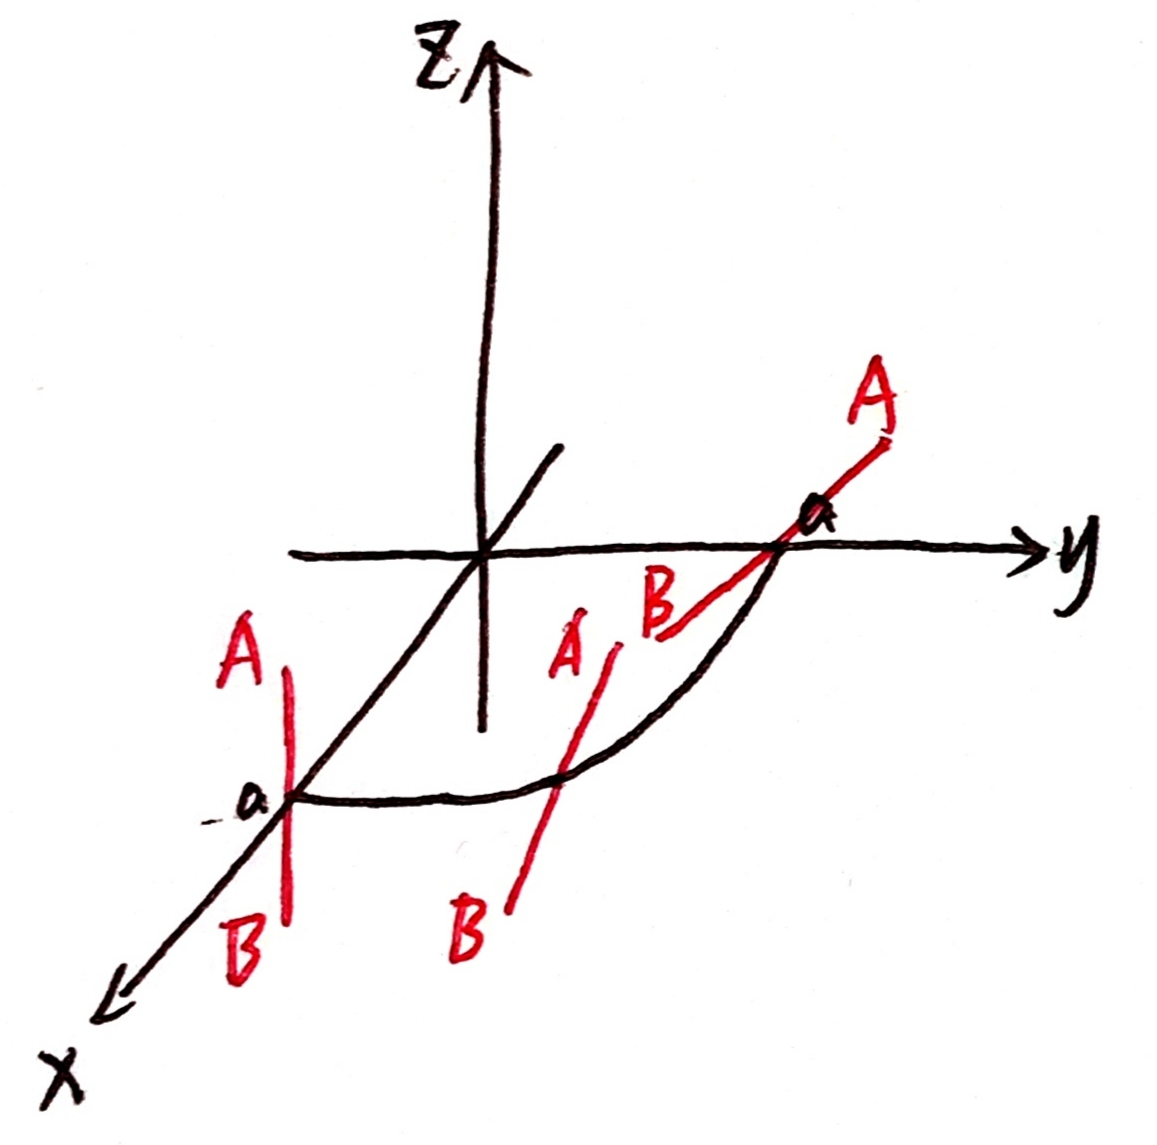
\includegraphics[width=0.23\textwidth]{figure/3.1.1-1} %图片的名称或者路径之中有空格会出问题 
 		\caption{$\R^3$ 中的$M\ddot{o}bius$ 带} % 图片标题
 		\label{pic 3.1.1-1}
 	\end{figure}
 
 	\newpage
 	下面我们构造一个从矩形纸带$X$ 到上述构造的$M\ddot{o}bius$ 带$M$ 的映射$\varphi : X \longrightarrow M$,使其实现直观上的\textbf{“粘合过程”}.
 	
 	\vspace{2em}
 	对于$M$ 上任一点,其只由公转的角度$\vartheta$ 和它与木棍中点的距离$u$ 决定,其中
 	\begin{align}
 		-l \leq u \leq l , \,\, 0 \leq \vartheta \leq 2\pi
 	\end{align}
	可以定义纸带即为$X = [0 , 2\pi] \times [-l , l]$, 从而不难得到
	\begin{align}
		\varphi : X &\longrightarrow M \\
		(\vartheta , u) &\longmapsto \left( (a + u\sin{\frac{\vartheta}{2}}) \cos{\vartheta} \,\, , \,\, (a + u\sin{\frac{\vartheta}{2}}) \sin{\vartheta} \,\, , \,\, u\cos{\frac{\vartheta}{2}} \right)
	\end{align}

	\begin{figure}[thbp!]
		\centering
		\begin{minipage}[t]{0.49\linewidth}
			\centering
			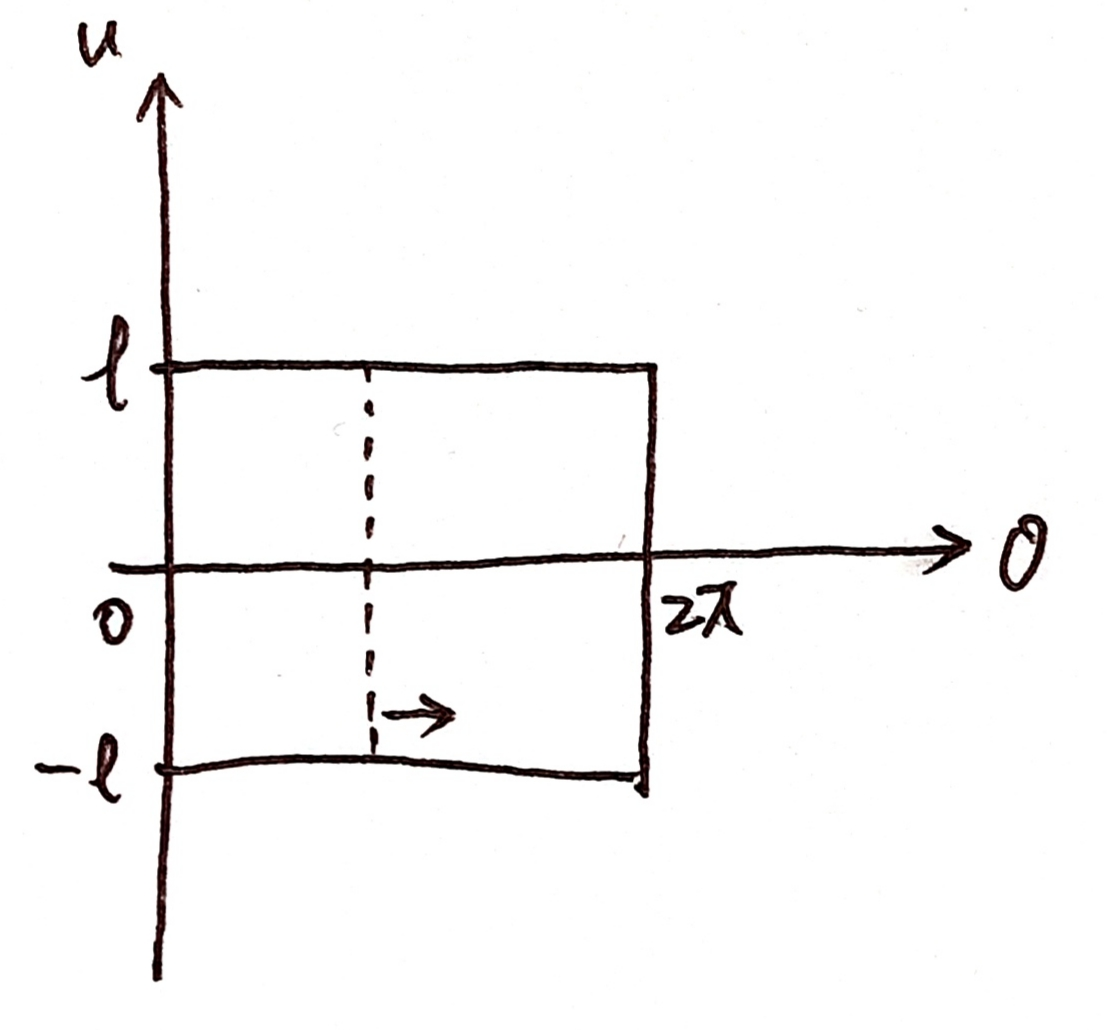
\includegraphics[width=0.5\linewidth]{figure/3.1.1-2}
			\caption\centering{\fontsize{10pt}{15pt}\selectfont{\songti}纸带$X$}
			\label{pic 3.1.1-2} % 添加图像引用标签
		\end{minipage}
		\begin{minipage}[t]{0.49\linewidth}
			\centering
			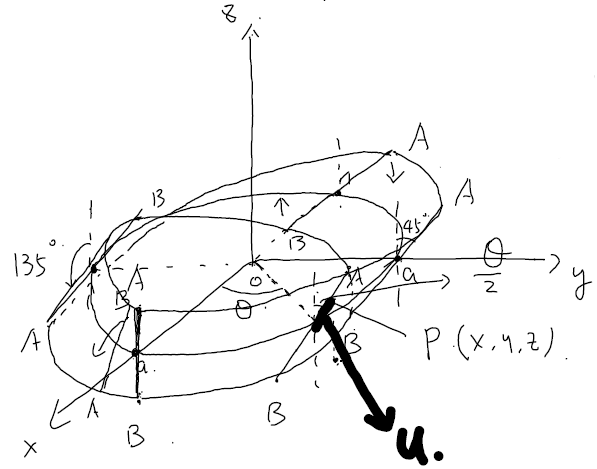
\includegraphics[width=0.7\linewidth]{figure/3.1.1-3}
			\caption\centering{\fontsize{10pt}{15pt}\selectfont{\songti}$\R^3$ 中的$M\ddot{o}bius$ 带}
			\label{pic 3.1.1-3} % 添加图像引用标签
		\end{minipage}
	\end{figure}

	容易得到,$\vartheta$ 增大,表示线段$\{ \vartheta \} \times [-l , l]$ 的像,即$M$ 中的木棍就在公转+自转.
	
	\vspace{2em}
	这样,我们就借助$\R^3$ 给出了$M\ddot{o}bius$ 带的表示形式,并定义了其拓扑空间. 但这样直观的方法自然而然存在着一个问题,就是这样定义\textbf{需要借助$\R^3$ 这个与$X$ 无关的第三方空间}.
	
	\vspace{1em}
	然而按理来说,$M\ddot{o}bius$ 带的构成应当只与我们的纸带$X$ 以及粘合方式有关,不应当依赖于第三方空间,这就引出了接下来讲的\textbf{抽象}方法.
	
\newpage
\paragraph{抽象方法}








	%  ############################
	\ifx\allfiles\undefined
\end{document}
\fi